% !TeX program = xelatex
% 物理学难题集萃 力学篇 · 题目部分（一页一题，无封面）
\documentclass[12pt,a4paper,openany]{book}

\usepackage{ctex}
\usepackage{amsmath,amssymb,amsthm}
\usepackage{esint}
\usepackage{geometry}
\geometry{left=2.2cm,right=2.2cm,top=2.2cm,bottom=2.2cm}
\usepackage{graphicx}
\usepackage{array}
\usepackage{fancyhdr}

\pagestyle{fancy}
\fancyhf{}
\fancyhead[L]{\small 物理学难题集萃（力学）}
\fancyhead[C]{\small\leftmark}
\fancyhead[R]{\small 力学}
\fancyfoot[C]{\thepage}
\renewcommand{\headrulewidth}{0.4pt}
\setlength{\headheight}{15pt}

\setlength{\parindent}{0pt}
\setlength{\parskip}{2pt}
\allowdisplaybreaks
\raggedbottom

\begin{document}

\chapter{运动学}
\textbf{1-1} 如力图1-1-1，直角三角形ABC在铅垂平面内，斜边AC与水平边BC的夹角为$\alpha$，一质点从A点由静止出发，在重力作用下到达C点。当所循路径为从A经AB和BC时，从A到B需时 $t_{1}$，从B到C需时 $t_{2}$；当所循路径为AC时需时 $t_{3}$，假定质点拐折时不花费时间，且只改变速度方向而速度大小不变。

1. 为使循上述两条路径由 $A$ 到 $C$ 所需时间相等，即使 $t_1 + t_2 = t_3$，试问角 $\alpha$ 应为多大？

2. 设角 $\alpha$ 取上述值，设质点只能在三角形范围内沿竖直路径和水平路径从 $A$ 点到达 $C$ 点，显然有无穷多种选择。试问什么路径花费的时间最多？什么路径花费的时间最少？所需的最长时间与最短时间之比是多少？



\begin{center}
\begin{tabular}{c}
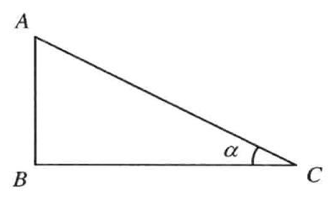
\includegraphics[width=0.3\linewidth,height=0.6\textheight,keepaspectratio]{figures/力图1-1-1.png}\\[2pt]
\textit{力图1-1-1}
\end{tabular}
\end{center}
\vfill
\newpage

\textbf{1-2} 一质点以初速度 $v_{0}$ 作直线运动，所受阻力与其速度成正比。试求当质点速度减为 $\dfrac{v_0}{n}$ $(n > 1)$ 时，质点经过的距离与质点所能行经的总距离之比。
\vfill
\newpage

\textbf{1-3} 一质点以初速度 $v_{0}$ 作直线运动，所受阻力与其速度的三次方成正比。试求质点速度和位置随时间的变化规律以及速度随位置的变化规律。
\vfill
\newpage

\textbf{1-4} 如力图1-4-1，在倾角为 $\theta$ 的山坡平面上有一门大炮，大炮相对于山坡的仰角为 $\alpha$，发射炮弹的初速为 $v_{0}$。试求炮弹着点的位置，并求能达到最大射程的仰角，忽略空气阻力。



\begin{center}
\begin{tabular}{c}
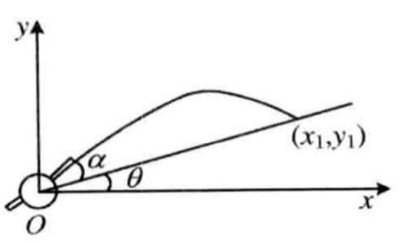
\includegraphics[width=0.3\linewidth,height=0.6\textheight,keepaspectratio]{figures/力图1-4-1.png}\\[2pt]
\textit{力图1-4-1}
\end{tabular}
\end{center}
\vfill
\newpage

\textbf{1-5} 两质点在地面上同一地点以相同速率 $v_{0}$ 从不同抛射角抛出。试证明，当两质点的射程 $R$ 相同时，它们在空中飞行时间的乘积为 $\dfrac{2R}{g}$，忽略空气阻力。

\begin{center}
\begin{tabular}{c}
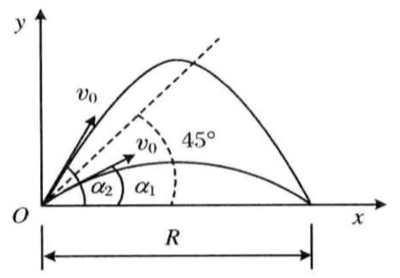
\includegraphics[width=0.3\linewidth,height=0.6\textheight,keepaspectratio]{figures/力图1-5-1.png}\\[2pt]
\textit{力图1-5-1}
\end{tabular}
\end{center}
\vfill
\newpage

\textbf{1-6} 如力图1-6-1，位于地面的水枪与一竖直墙的垂直距离为 $d = 3.0\,\mathrm{m}$，墙高 $h = 4.0\,\mathrm{m}$。从水枪喷出初速恒定的水流，为使水流刚好能越过墙顶，试问水流从枪口喷出的初速 $v_{0}$ 的最小值以及水枪的仰角 $\alpha$ 各为多少？忽略空气阻力，重力加速度 $g$ 取 $10\,\mathrm{m/s^2}$。



\begin{center}
\begin{tabular}{c}
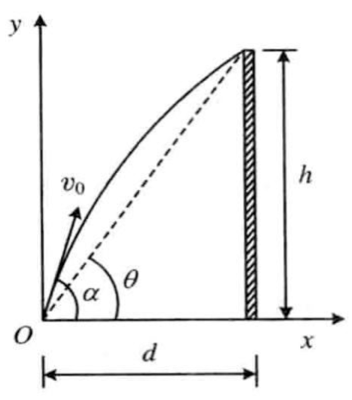
\includegraphics[width=0.3\linewidth,height=0.6\textheight,keepaspectratio]{figures/力图1-6-1.png}\\[2pt]
\textit{力图1-6-1}
\end{tabular}
\end{center}
\vfill
\newpage

\textbf{1-7} 如力图1-7-1，球1和球2均从同一点水平抛出，起抛点离水平地面的高度为 $H$。两球的水平初速分别为 $v_{1}$ 和 $v_{2}$ $(v_{1} > v_{2})$。球1抛出后刚好能越过位于 $x_{P}$ 处的竖直杆的顶端，并落于地面上的 $R$ 点，$R$ 点与 $O$ 点的距离为 $R$。球2抛出后落于地面，与地面作弹性碰撞，反弹后也刚好越过杆顶，并落在同一点 $R$。试求：1. 比值 $\dfrac{v_1}{v_2}$。2. 杆的位置 $x_{P}$。3. 杆的高度 $h$。



\begin{center}
\begin{tabular}{c}
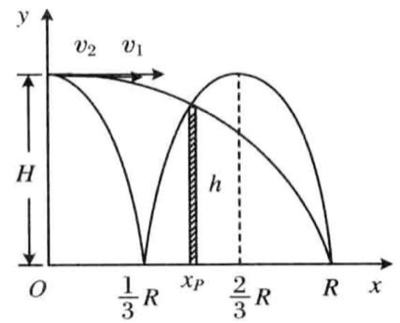
\includegraphics[width=0.3\linewidth,height=0.6\textheight,keepaspectratio]{figures/力图1-7-1.png}\\[2pt]
\textit{力图1-7-1}
\end{tabular}
\end{center}
\vfill
\newpage

\textbf{1-8} 飞行物自地面以匀速 $v_{\mathrm{f}}$ 向上空垂直飞行。在地面离飞行物起飞点相距 $L$ 处发射一枚导弹，导弹与飞行物同时发射。导弹的速率 $v$ 为常值，且 $v > v_{\mathrm{f}}$，每一瞬时导弹均指向飞行物运动。

1. 试求导弹的飞行轨迹；

2. 试问导弹经多长时间击中飞行物。

\begin{center}
\begin{tabular}{c}
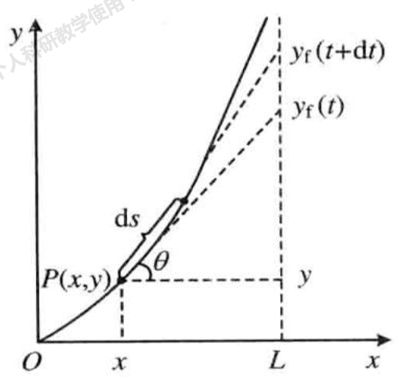
\includegraphics[width=0.3\linewidth,height=0.6\textheight,keepaspectratio]{figures/力图1-8-1.png}\\[2pt]
\textit{力图1-8-1}
\end{tabular}
\end{center}
\vfill
\newpage

\textbf{1-9} 圆柱体固定不动，其轴线与水平面垂直。很轻的不可伸长的柔软细线全部缠绕在圆柱体上且在同一水平面内，线末端系一小球，紧贴圆柱体表面。突然给小球一击，使之具有在水平方向并与圆柱体垂直的初速度 $\boldsymbol{v}$，于是缠绕的细线开始从圆柱体上解开。设解开过程中细线与圆柱体之间无相对滑动，且重力可略，即小球始终在水平面内运动。

试求：1. 小球的加速度。2. 小球的轨迹方程。

\begin{center}
\begin{tabular}{c}
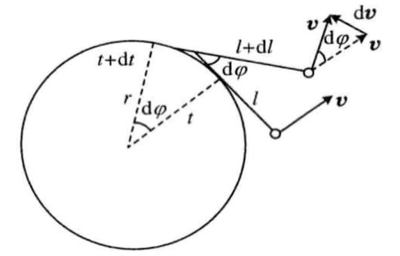
\includegraphics[width=0.3\linewidth,height=0.6\textheight,keepaspectratio]{figures/力图1-9-1.png}\\[2pt]
\textit{力图1-9-1}
\end{tabular}
\end{center}
\vfill
\newpage

\textbf{1-10} 细杆绕端点 $O$ 在平面内匀角速旋转，角速度为 $\omega$，杆上一小环（可看作质点）相对杆作匀速运动，相对速度为 $v$。设 $t = 0$ 时刻小环位于杆的端点 $O$。

1. 试证明小环的运动轨迹为阿基米德螺线。

2. 试求小环在任意时刻的速度和加速度。

3. 试用作图法定性画出小环加速度在自然坐标系中的两个分量（切向加速度和法向加速度）。

\begin{center}
\begin{tabular}{c}
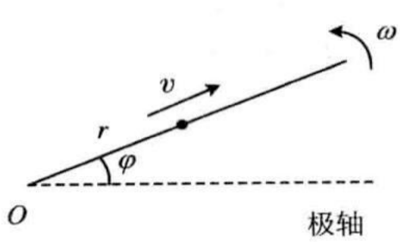
\includegraphics[width=0.3\linewidth,height=0.6\textheight,keepaspectratio]{figures/力图1-10-1.png}\\[2pt]
\textit{力图1-10-1}
\end{tabular}
\end{center}
\vfill
\newpage

\textbf{1-11} 如力图1-11-1所示，质点 $A$ 和质点 $B$ 同时从 $A$、$B$ 两点出发，分别以速度 $v_{1}$ 沿 $AB$ 和以速度 $v_{2}$ 沿 $BC$ 作匀速直线运动，$BC$ 和 $AB$ 的夹角为 $\alpha$，开始时质点 $A$ 和质点 $B$ 相距为 $l$，试求两质点之间的最短距离。



\begin{center}
\begin{tabular}{c}
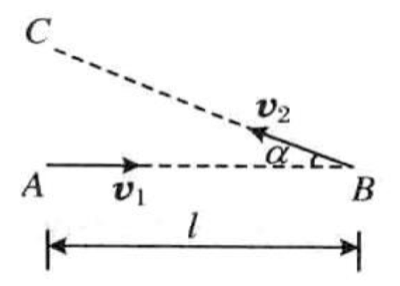
\includegraphics[width=0.3\linewidth,height=0.6\textheight,keepaspectratio]{figures/力图1-11-1.png}\\[2pt]
\textit{力图1-11-1}
\end{tabular}
\end{center}
\vfill
\newpage

\textbf{1-12} 宽 $L$ 的河流，流速与离岸的距离成正比，已知两岸处的流速为零，河中心的流速为 $v_{0}$。一小船以恒定的相对速度 $v_{r}$ 垂直于水流从一岸驶向另一岸。在离岸 $\dfrac{L}{4}$ 处因故突然掉头，以相对速度 $\dfrac{v_{r}}{2}$ 垂直于水流驶回本岸。

试求：1. 小船的运动轨迹。2. 小船返回本岸时，所到处与原出发点的距离是多少。

\begin{center}
\begin{tabular}{c}
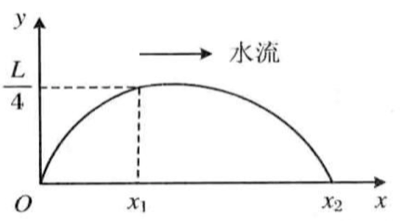
\includegraphics[width=0.3\linewidth,height=0.6\textheight,keepaspectratio]{figures/力图1-12-1.png}\\[2pt]
\textit{力图1-12-1}
\end{tabular}
\end{center}
\vfill
\newpage

\textbf{1-13} 如力图1-13-1，一条笔直的河流宽度为 $d$，河水以恒定的速度 $v_{0}$ 流动。小船从河岸的 $A$ 点出发，为了到达对岸的 $O$ 点，相对于河水以恒定的速率 $v^{\prime}$ $(v^{\prime} > v_{0})$ 运动，不论小船驶到何处，它的运动方向总是指向 $O$ 点。已知 $\overline{AO} = r_0$，$\angle AOP = \varphi_0$，试求小船运动的轨迹。若 $O$ 点刚好在 $A$ 点的对面（即 $\overline{AO} = d$），结果又如何？



\begin{center}
\begin{tabular}{c}
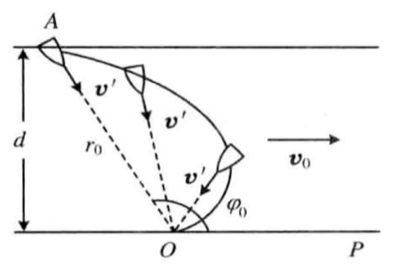
\includegraphics[width=0.3\linewidth,height=0.6\textheight,keepaspectratio]{figures/力图1-13-1.png}\\[2pt]
\textit{力图1-13-1}
\end{tabular}
\end{center}
\vfill
\newpage

\textbf{1-14} 如力图1-14-1，轮子在水平面上以角速度 $\omega$ 作纯滚动，已知轮子的质心速度为 $v_{\mathrm{c}}$，试求轮边缘上任一点 $A$ 的绝对速度，$A$ 点的位置用 $\theta$ 角表示。



\begin{center}
\begin{tabular}{c}
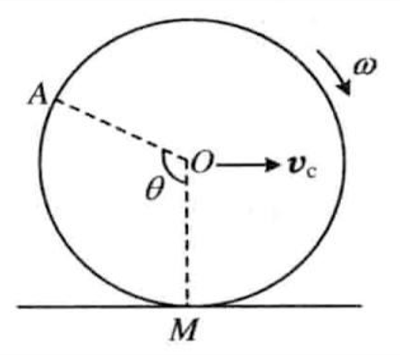
\includegraphics[width=0.3\linewidth,height=0.6\textheight,keepaspectratio]{figures/力图1-14-1.png}\\[2pt]
\textit{力图1-14-1}
\end{tabular}
\end{center}
\vfill
\newpage

\textbf{1-15} 如力图1-15-1，半径为 $R$ 的圆环静止不动，半径为 $r$ 的圆盘沿圆环内侧作无滑动的滚动，圆盘中心 C 点绕环中心 O 点的角速度恒为 $\Omega$。试求圆盘上与圆环相接触的 A 点相对圆环的加速度。



\begin{center}
\begin{tabular}{c}
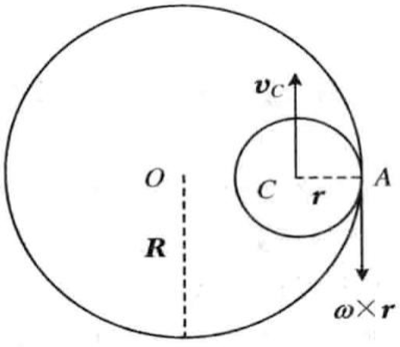
\includegraphics[width=0.3\linewidth,height=0.6\textheight,keepaspectratio]{figures/力图1-15-1.png}\\[2pt]
\textit{力图1-15-1}
\end{tabular}
\end{center}
\vfill


\chapter{牛顿运动定律}
\textbf{2-1} 如力图2-1-1，在固定不动的圆柱体上绕有绳索，绳两端挂大、小两桶，其质量分别为 $M = 1000\,\mathrm{kg}$ 和 $m = 10\,\mathrm{kg}$。绳与圆柱体之间的摩擦系数为 $\mu = 0.050$，绳的质量可以忽略。试问为使两桶静止不动，绳至少需绕多少圈。



\begin{center}
\begin{tabular}{c}
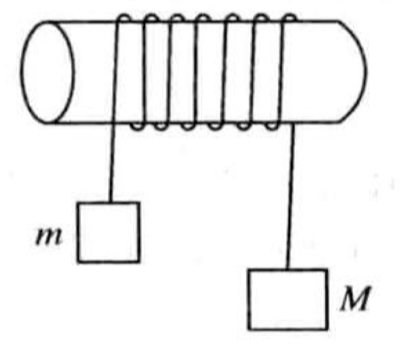
\includegraphics[width=0.3\linewidth,height=0.6\textheight,keepaspectratio]{figures/力图2-1-1.png}\\[2pt]
\textit{力图2-1-1}
\end{tabular}
\end{center}
\vfill
\newpage

\textbf{2-2} 如力图2-2-1，细杆一端支在地面上，以恒定的角速度 $\omega$ 绕通过支点的竖直轴旋转，杆与地面的夹角为 $\alpha$，质量为 $m$ 的小环套在杆上，可以沿杆滑动，环与杆之间的摩擦系数为 $\mu$。试问小环处于什么位置上能维持稳定运动。



\begin{center}
\begin{tabular}{c}
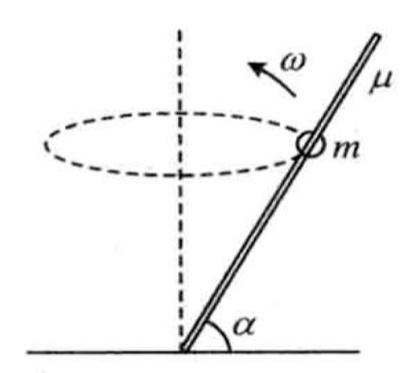
\includegraphics[width=0.3\linewidth,height=0.6\textheight,keepaspectratio]{figures/力图2-2-1.png}\\[2pt]
\textit{力图2-2-1}
\end{tabular}
\end{center}
\vfill
\newpage

\textbf{2-3} 如力图2-3-1，在半径为 $R$ 的空心球壳内壁，有一可当作质点的小球沿固定的水平圆周作匀速率运动，小球与空心球壳球心的连线与铅垂线的夹角为 $\theta$，小球与空心球壳内壁之间的摩擦系数为 $\mu$。试求小球能稳定运动的速度范围。



\begin{center}
\begin{tabular}{c}
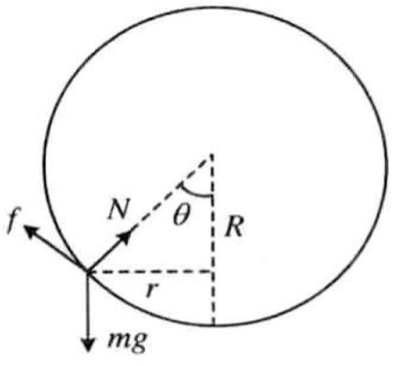
\includegraphics[width=0.3\linewidth,height=0.6\textheight,keepaspectratio]{figures/力图2-3-1.png}\\[2pt]
\textit{力图2-3-1}
\end{tabular}
\end{center}
\vfill
\newpage

\textbf{2-4} 如力图2-4-1，在地面上有一倾角为 $\theta$、质量为 $M$ 的斜面体，斜面体上有一质量为 $m$ 的木块，设地面与斜面体之间以及斜面体与木块之间均光滑无摩擦。试求 $M$ 与 $m$ 相对于地面的加速度 $a_{M}$ 与 $a_{m}$，以及木块 $m$ 所受的支持力。



\begin{center}
\begin{tabular}{c}
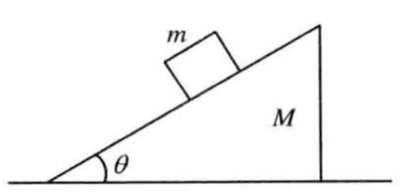
\includegraphics[width=0.3\linewidth,height=0.6\textheight,keepaspectratio]{figures/力图2-4-1.png}\\[2pt]
\textit{力图2-4-1}
\end{tabular}
\end{center}
\vfill
\newpage

\textbf{2-5} 如力图2-5-1，一个半径为 $R = 0.5\,\mathrm{m}$ 的空心球壳绕本身的竖直直径旋转，角速度为 $\omega = 5\,\mathrm{s^{-1}}$，在空心球壳内高度为 $\dfrac{R}{2}$ 处有一小木块（可当作质点）同球壳一起旋转。

试求：1. 摩擦系数至少是多少才能实现这一情况。2. 当 $\omega = 8\,\mathrm{s^{-1}}$ 时，实现这一情况的条件是什么。3. 研究以下两种情形运动的稳定性：(a) 木块位置有微小变动；(b) 空心球壳的角速度有微小变动。



\begin{center}
\begin{tabular}{c}
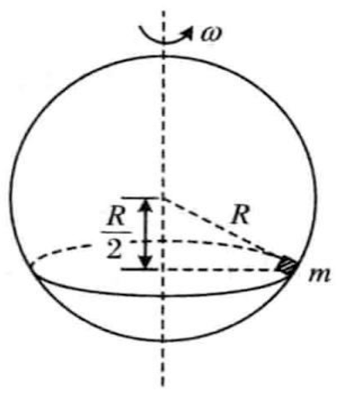
\includegraphics[width=0.3\linewidth,height=0.6\textheight,keepaspectratio]{figures/力图2-5-1.png}\\[2pt]
\textit{力图2-5-1}
\end{tabular}
\end{center}
\vfill
\newpage

\textbf{2-6} 如力图2-6-1，一质量为 $m = 20\,\mathrm{kg}$ 的对称钢件，架在两个完全相同的平行长直滚轴上。两滚轴在同一水平面内，滚轴半径为 $r = 0.025\,\mathrm{m}$，绕各自的中心轴以相同的角速度 $\omega = 40\,\mathrm{rad/s}$ 作反向转动。钢件与滚轴间的摩擦系数为 $\mu = 0.20$。为使钢件以 $v_{0} = 0.050\,\mathrm{m/s}$ 的速度沿滚轴作匀速直线运动，需沿滚轴的长度方向对钢件施以水平作用力 $F$，试求 $F$ 的大小。



\begin{center}
\begin{tabular}{c}
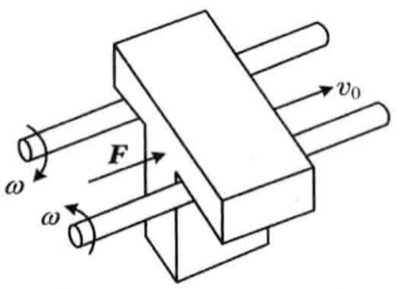
\includegraphics[width=0.3\linewidth,height=0.6\textheight,keepaspectratio]{figures/力图2-6-1.png}\\[2pt]
\textit{力图2-6-1}
\end{tabular}
\end{center}
\vfill
\newpage

\textbf{2-7} 如力图2-7-1所示，质量分别为 $m_{A}$ 和 $m_{B}$ 的两木块 A 和 B 静止放置在粗糙的水平地面上，两者与地面之间的摩擦系数均为 $\mu$，两木块 A 和 B 的接触面是倾角为 $\theta$ 的斜面，接触面是光滑的。现施一水平推力 $F$ 于 A，使 A 和 B 产生向右的加速度，且 A 和 B 之间不发生相对滑动。试问 $\mu$ 和 $F$ 各应满足什么条件。



\begin{center}
\begin{tabular}{c}
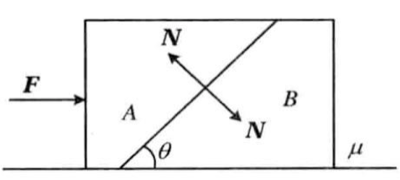
\includegraphics[width=0.3\linewidth,height=0.6\textheight,keepaspectratio]{figures/力图2-7-1.png}\\[2pt]
\textit{力图2-7-1}
\end{tabular}
\end{center}
\vfill
\newpage

\textbf{2-8} 如力图2-8-1所示，质量为 $M$ 的滑块C放置在光滑桌面上。质量均为 $m$ 的两个重物 A 和 B 用细绳相连，A 平放在滑块上，与滑块间的摩擦系数为 $\mu$，细绳跨过滑轮后将 B 竖直悬挂。设细绳和滑轮的质量均忽略不计，滑轮转轴不受摩擦力。今以水平推力 $F$ 作用于滑块，为使重物 A 和 B 与滑块保持相对静止，试问 $F$ 至少应多大？



\begin{center}
\begin{tabular}{c}
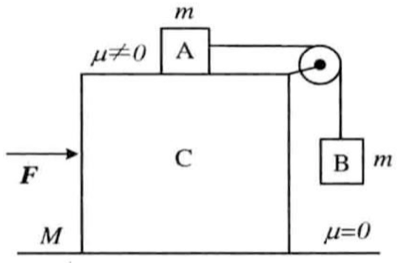
\includegraphics[width=0.3\linewidth,height=0.6\textheight,keepaspectratio]{figures/力图2-8-1.png}\\[2pt]
\textit{力图2-8-1}
\end{tabular}
\end{center}
\vfill
\newpage

\textbf{2-9} 如力图2-9-1所示，在水平面内有一平台可绕竖直的中心轴以角速度 $\omega$ 匀角速旋转，在平台内沿半径方向有一光滑细槽，槽内放置两质量均为 $m$ 的小球，两球用劲度系数为 $k$、原长为 $a$ 的轻弹簧相连。弹簧的自然长度恰好等于槽的宽度，即两球刚好接触。平台以角速度 $\omega$ 旋转时，两球在槽内离中心的距离分别为 $r_{1}$ 和 $r_{2}$，试求 $r_{1}$ 和 $r_{2}$。



\begin{center}
\begin{tabular}{c}
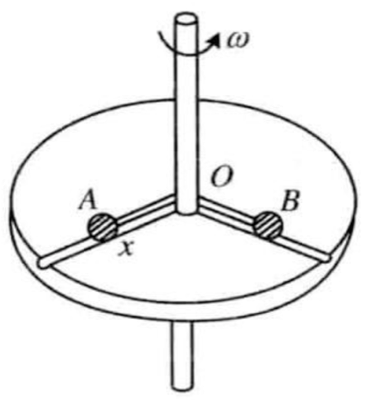
\includegraphics[width=0.3\linewidth,height=0.6\textheight,keepaspectratio]{figures/力图2-9-1.png}\\[2pt]
\textit{力图2-9-1}
\end{tabular}
\end{center}
\vfill
\newpage

\textbf{2-10} 质量为 $m$ 的物体以初速 $v_{0}$ 从地面竖直上抛，设空气阻力 $f = \mu v^{2}$，$\mu$ 为常数。试求物体达到的最大高度，并证明物体返回原处的速度为 $v_{0}\sqrt{\dfrac{mg}{mg + \mu v_{0}^{2}}}$。

\begin{center}
\begin{tabular}{c}
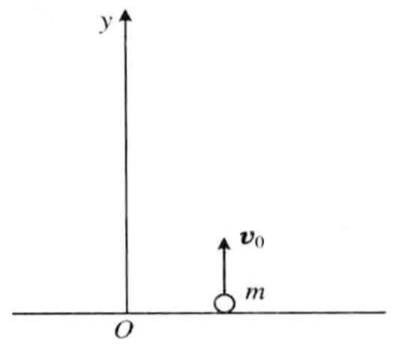
\includegraphics[width=0.3\linewidth,height=0.6\textheight,keepaspectratio]{figures/力图2-10-1.png}\\[2pt]
\textit{力图2-10-1}
\end{tabular}
\end{center}
\vfill
\newpage

\textbf{2-11} 两质点的质量均为 $m$，质点1从离地面高度为 $h$ 处由静止下落，质点2从质点1正下方的地面上以初速 $v_0$ 同时竖直上抛。设空气阻力与质点速率成正比，比例系数为 $\mu$（常量）。试求两质点相遇的时间、地点以及相遇时两质点的速度。

\begin{center}
\begin{tabular}{c}
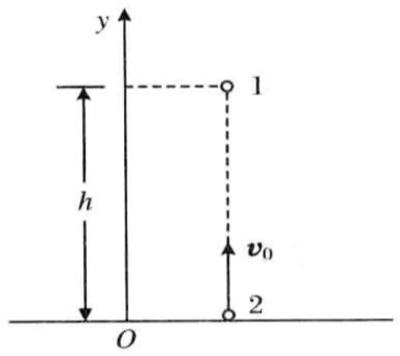
\includegraphics[width=0.3\linewidth,height=0.6\textheight,keepaspectratio]{figures/力图2-11-1.png}\\[2pt]
\textit{力图2-11-1}
\end{tabular}
\end{center}
\vfill
\newpage

\textbf{2-12} 质量为 $m$ 的抛射体初速为 $v_{0}$，抛射角为 $\alpha$，在空气中运动时，所受阻力与速率成正比，比例系数为 $k$。试求轨迹方程，并验证当 $k \to 0$ 时变为抛物方程。

\begin{center}
\begin{tabular}{c}
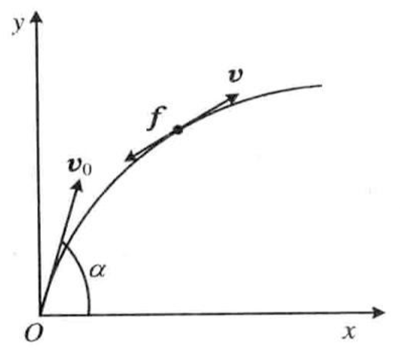
\includegraphics[width=0.3\linewidth,height=0.6\textheight,keepaspectratio]{figures/力图2-12-1.png}\\[2pt]
\textit{力图2-12-1}
\end{tabular}
\end{center}
\vfill
\newpage

\textbf{2-13} 飞机以 $v_{0} = 90\,\mathrm{km/h}$ 的水平速度触地滑行着陆。滑行期间受到的空气阻力为 $c_{x}v^{2}$，升力与速度平方成正比，即 $L = c_{y}v^{2}$。已知飞机质量为 $m$，机翼面积为 $S$，升阻比 $K = \dfrac{c_y}{c_x} = 5$，触地瞬间升力与重力恰好平衡。试求飞机触地后的滑行距离 $x$ 和速度随时间的变化关系 $v(t)$。
\vfill
\newpage

\textbf{2-14} 如力图2-14-1，质量为 $m$ 的小球用一质量可略的弹簧1竖直悬挂起来，弹簧的劲度系数为 $k$。当弹簧的伸长量超过临界长度 $l_{\mathrm{C}}$ $\left(l_{\mathrm{C}} > \dfrac{mg}{k}\right)$ 时，弹簧将被拉断。在小球下方再挂完全相同的另一弹簧2，并在其下端施一与时间 $t$ 有关的拉力 $F(t)$。若以小球在平衡位置时作为计时起点，则拉力随时间变化的关系为 $F(t) = \alpha t$，其中 $\alpha$ 是一恒定参量。试求两弹簧同时被拉断时，参量 $\alpha$ 应满足的关系式。



\begin{center}
\begin{tabular}{c}
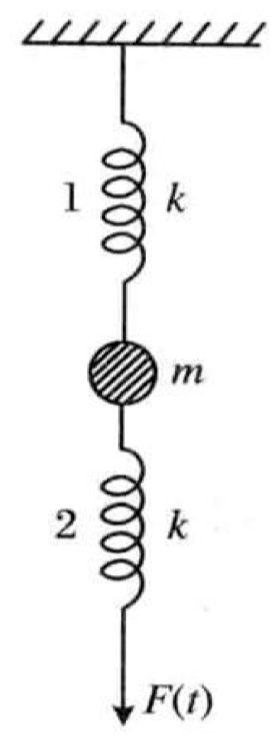
\includegraphics[width=0.3\linewidth,height=0.6\textheight,keepaspectratio]{figures/力图2-14-1.png}\\[2pt]
\textit{力图2-14-1}
\end{tabular}
\end{center}
\vfill
\newpage

\textbf{2-15} 如力图2-15-1，质量为 $M$、倾角为 $\theta$ 的斜面体放在光滑的桌面上，斜面体上有质量为 $m$ 的木块，木块与斜面体之间的摩擦系数 $\mu < \tan \theta$，以水平力 $F$ 推斜面体，使之运动。试问为了使木块相对于斜面体保持静止，$F$ 的大小应在什么范围。



\begin{center}
\begin{tabular}{c}
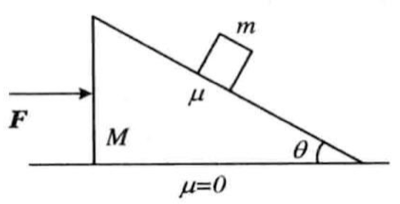
\includegraphics[width=0.3\linewidth,height=0.6\textheight,keepaspectratio]{figures/力图2-15-1.png}\\[2pt]
\textit{力图2-15-1}
\end{tabular}
\end{center}
\vfill
\newpage

\textbf{2-16} 如力图2-16-1，地面上有一质量为 $M$、倾角为 $\alpha_{1}$、$\alpha_{2}$ 的斜面体。质量为 $m_{1}$ 和 $m_{2}$ 的两木块分别置于斜面体两侧，用绳经滑轮相连。设地面、斜面、滑轮的摩擦以及绳子和滑轮的质量均可忽略，绳不可伸长，试求 $m_{1}$（或 $m_{2}$）相对 $M$ 的加速度以及 $M$ 的绝对加速度。



\begin{center}
\begin{tabular}{c}
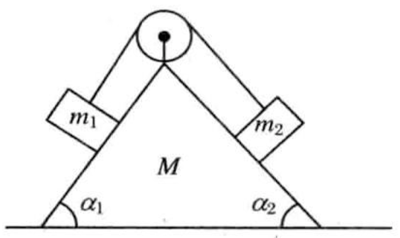
\includegraphics[width=0.3\linewidth,height=0.6\textheight,keepaspectratio]{figures/力图2-16-1.png}\\[2pt]
\textit{力图2-16-1}
\end{tabular}
\end{center}
\vfill
\newpage

\textbf{2-17} 如力图2-17-1，质量为 $m_{1}$ 的航天飞机A绕地球作匀速圆周运动，轨道半径为 $R$，从航天飞机伸出一长度为 $L$ $(L \ll R)$ 的刚性杆，杆端固定一质量为 $m_{2}$ $(m_{2} \ll m_{1})$ 的卫星S。设A和S均可看作质点，A-S系统的位置用 $\alpha$ 角表示，$\alpha$ 角是杆与A和地心连线之间的夹角。试求A-S系统的平衡位置，并讨论平衡的稳定性。



\begin{center}
\begin{tabular}{c}
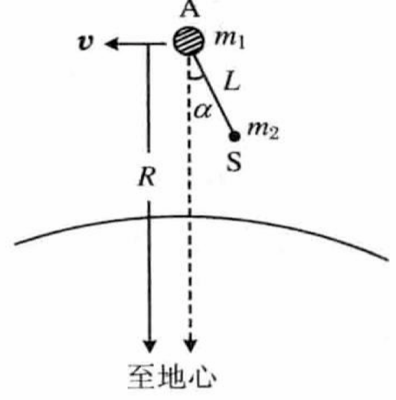
\includegraphics[width=0.3\linewidth,height=0.6\textheight,keepaspectratio]{figures/力图2-17-1.png}\\[2pt]
\textit{力图2-17-1}
\end{tabular}
\end{center}
\vfill
\newpage

\textbf{2-18} 如力图2-18-1，半径为 $R$ 的圆盘与水平面平行，绕通过盘中心 $O$ 的竖直轴以角速度 $\omega$ 匀速旋转。盘边缘 $A$ 点处的射手相对于圆盘以水平初速 $v_{0}$ 发射子弹，目标是直径 $AB$ 的另一端点 $B$。设子弹速度远大于盘的转速，且发射子弹不影响圆盘的角速度，设空气阻力可忽略。试问射手应瞄准何方才能击中目标？从射手看来，子弹的轨迹如何？



\begin{center}
\begin{tabular}{c}
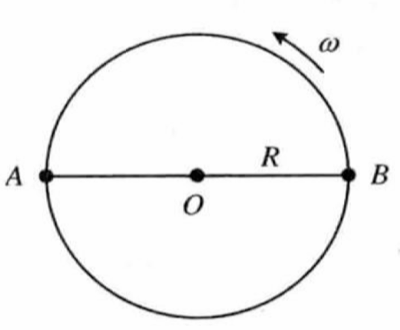
\includegraphics[width=0.3\linewidth,height=0.6\textheight,keepaspectratio]{figures/力图2-18-1.png}\\[2pt]
\textit{力图2-18-1}
\end{tabular}
\end{center}
\vfill
\newpage

\textbf{2-19} 地球以角速度 $\omega$ 自转，一质点在纬度 $\varphi$ 上空 $h$ 高度处自由下落。忽略空气阻力和惯性离心力。试求因科里奥利力引起的落地点的偏离。
\vfill
\newpage

\textbf{2-20} 1851年，法国物理学家傅科发现单摆并不在固定的平面内摆动。如果把每次摆动近似看作在一个平面内，并把这个平面称为摆动平面，则摆动平面将以一定角速度作缓慢的顺时针转动（在北半球）。这个现象是由地球的自转造成的，这种摆称为傅科摆。试证明傅科摆摆动平面的旋转周期 $T'$ 与摆所在处的纬度 $\varphi$ 有关，并遵守

\[
T' = \frac{T_0}{\sin\varphi}
\]

式中 $T_0 = \dfrac{2\pi}{\omega}$ 为地球自转周期。
\vfill


\chapter{功、能和动量}
\textbf{3-1} 如力图3-1-1，劲度系数为 $k$ 的弹簧下端竖直悬挂着两个物体，质量分别为 $m_{1}$ 和 $m_2$。达到平衡后，突然撤去 $m_{2}$，试求 $m_{1}$ 运动的最大速度。



\begin{center}
\begin{tabular}{c}
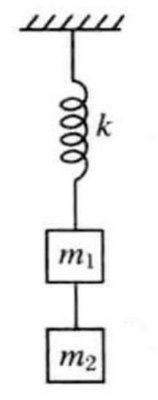
\includegraphics[width=0.3\linewidth,height=0.6\textheight,keepaspectratio]{figures/力图3-1-1.png}\\[2pt]
\textit{力图3-1-1}
\end{tabular}
\end{center}
\vfill
\newpage

\textbf{3-2} 如力图3-2-1，水平弹簧一端固定，另一端系一质量为 $m$ 的小球，弹簧的劲度系数为 $k$，小球与水平面之间的摩擦系数为 $\mu$。当弹簧为原长时小球位于 O 点，开始时小球位于 O 点右方的 A 点，O 与 A 之间的距离为 $l_{0}$，从静止释放小球。

1. 为使小球能通过 O 点，而且只能通过 O 点一次，试问 $\mu$ 值应在什么范围？

2. 在上述条件下，小球在 O 点左方的停住点 B 点与 O 点的最大距离 $l_{1}$ 是多少？



\begin{center}
\begin{tabular}{c}
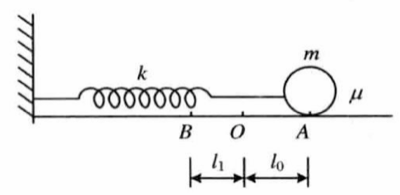
\includegraphics[width=0.3\linewidth,height=0.6\textheight,keepaspectratio]{figures/力图3-2-1.png}\\[2pt]
\textit{力图3-2-1}
\end{tabular}
\end{center}
\vfill
\newpage

\textbf{3-3} 如力图3-3-1所示，一木块沿倾角 $\theta = 30^{\circ}$ 的斜面从某初始位置以 $v_{0} = 4.5\,\mathrm{m/s}$ 的初速向上运动。已知木块与斜面之间的摩擦系数 $\mu = 0.35$。规定木块初始位置处的重力势能为零。试求木块动能等于重力势能处相对其初始位置的高度。


\begin{center}
\begin{tabular}{c}
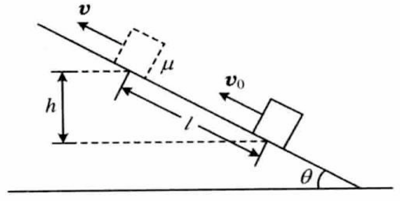
\includegraphics[width=0.3\linewidth,height=0.6\textheight,keepaspectratio]{figures/力图3-3-1.png}\\[2pt]
\textit{力图3-3-1}
\end{tabular}
\end{center}
\vfill
\newpage

\textbf{3-4} 如力图3-4-1，在水平桌面上开有一孔，绳子的一部分平放在桌面上，另一部分经孔下垂。设绳不可伸长，均匀柔软，全长为 $l$，下垂长度为 $x_0$，从静止开始下落。设摩擦可略。试求在下落过程中，绳子速度随下落长度变化的规律，以及绳的下端位置随时间变化的规律。


\begin{center}
\begin{tabular}{c}
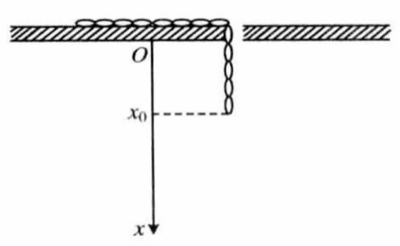
\includegraphics[width=0.3\linewidth,height=0.6\textheight,keepaspectratio]{figures/力图3-4-1.png}\\[2pt]
\textit{力图3-4-1}
\end{tabular}
\end{center}
\vfill
\newpage

\textbf{3-5} 如力图3-5-1，单摆的摆长为 $L$，摆球质量为 $m$，从左侧与竖直方向夹角 $\alpha$ 处静止下摆。在右侧，与悬点相距为 $r$、与竖直方向夹角为 $\beta$ $(\beta < \alpha)$ 处有一固定的钉子。设空气阻力可略。

试求：1. 为使小球能绕钉子作一个完整的圆周运动，角 $\alpha$ 至少应多大？2. 为使小球能与钉子相碰，角 $\alpha$ 应多大？



\begin{center}
\begin{tabular}{c}
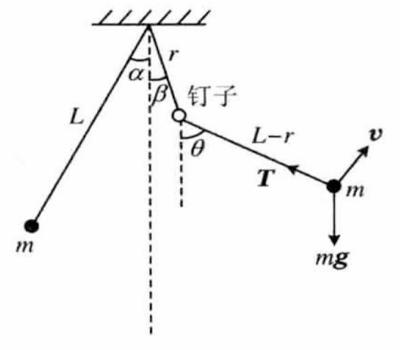
\includegraphics[width=0.3\linewidth,height=0.6\textheight,keepaspectratio]{figures/力图3-5-1.png}\\[2pt]
\textit{力图3-5-1}
\end{tabular}
\end{center}
\vfill
\newpage

\textbf{3-6} 如力图3-6-1，质量为 $M$ 的圆环用细线（质量可略）悬挂，圆环上串着两个质量均为 $m$ 的小球，两小球自圆环顶端从静止开始同时向两边滑下，设摩擦可略。



\begin{center}
\begin{tabular}{c}
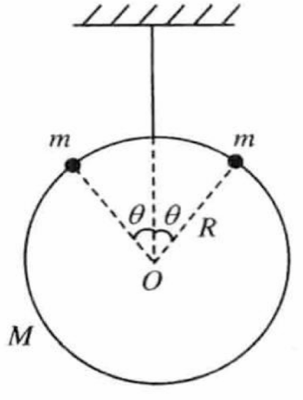
\includegraphics[width=0.3\linewidth,height=0.6\textheight,keepaspectratio]{figures/力图3-6-1.png}\\[2pt]
\textit{力图3-6-1}
\end{tabular}
\end{center}
\vfill
\newpage

\textbf{3-7} 如力图3-7-1，长为 $2r = 20\,\mathrm{cm}$、质量可以忽略的棒，中心点 $C$ 处有一固定的质量为 $m$ 的质点。棒一端 $A$ 点靠在竖直墙上，另一端 $B$ 点支在地面上，两端可分别沿墙和地面无摩擦地滑动。棒从竖直位置静止下滑，滑动过程中棒始终保持在同一竖直平面内。试求棒中心 $C$ 点触地的位置。



\begin{center}
\begin{tabular}{c}
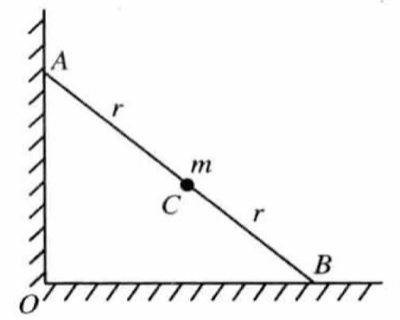
\includegraphics[width=0.3\linewidth,height=0.6\textheight,keepaspectratio]{figures/力图3-7-1.png}\\[2pt]
\textit{力图3-7-1}
\end{tabular}
\end{center}
\vfill
\newpage

\textbf{3-8} 如力图3-8-1所示，长为 $L$ 的细杆顶端固定一小重球，竖直倒置在粗糙的水平地面上。小球处于不稳定的平衡状态，稍有扰动，小球将从静止开始向下跌落。假设细杆很轻，其质量可略。试求小球碰地时速度的水平分量和竖直分量。



\begin{center}
\begin{tabular}{c}
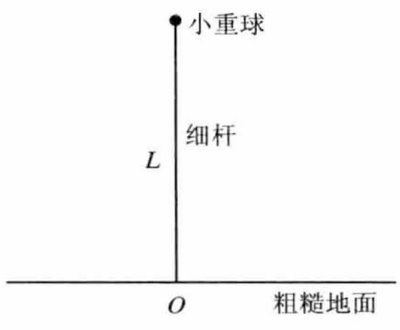
\includegraphics[width=0.3\linewidth,height=0.6\textheight,keepaspectratio]{figures/力图3-8-1.png}\\[2pt]
\textit{力图3-8-1}
\end{tabular}
\end{center}
\vfill
\newpage

\textbf{3-9} 如力图3-9-1，长为 $2l$ 的不可伸长的细绳一端固定于 $A$ 点的钉子上，另一端系一小球，小球可绕 $A$ 点在铅垂面内运动。开始时小球与 $A$ 点位于同一水平线上，小球在 $A$ 点右侧，垂直向下的初速度为 $v_{0}$。与 $A$ 点在同一水平线上左侧的 $B$ 点也有一钉子，$A$ 与 $B$ 之间的距离为 $l$。当细绳转到 $B$ 点后，小球将绕 $B$ 点向上运动。为使小球能与 $A$ 点的钉子相碰，试问小球初速 $v_{0}$ 的最小值应为多少？

\begin{center}
\begin{tabular}{c}
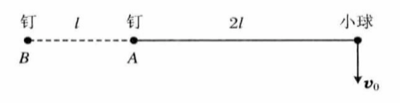
\includegraphics[width=0.3\linewidth,height=0.6\textheight,keepaspectratio]{figures/力图3-9-1.png}\\[2pt]
\textit{力图3-9-1}
\end{tabular}
\end{center}
\vfill
\newpage

\textbf{3-10} 如力图3-10-1所示，在惯性系 $S$ 中有两质点 $A$ 和 $B$，质量分别为 $m_{1}$ 和 $m_{2}$，彼此间以万有引力相互吸引。开始时 $A$ 静止，$A$ 和 $B$ 相距 $l_{0}$，$B$ 以速度 $v_{0}$ 沿连线方向远离 $A$ 而运动 $(v_{0} < \sqrt{\frac{2Gm_2}{l_0}})$，$G$ 为引力常量。$B$ 受一指向其运动方向的变力 $F$ 的作用，使 $B$ 保持速度 $v_{0}$ 不变。

试求：1. 两质点之间的最大距离 $l_{\max}$。2. 从开始到最大距离过程中，变力 $F$ 所作的功（相对于惯性系 $S$）。



\begin{center}
\begin{tabular}{c}
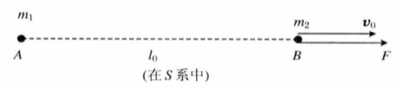
\includegraphics[width=0.3\linewidth,height=0.6\textheight,keepaspectratio]{figures/力图3-10-1.png}\\[2pt]
\textit{力图3-10-1}
\end{tabular}
\end{center}
\vfill
\newpage

\textbf{3-11} 如力图3-11-1，设想在地球表面的 $A$、$B$ 两地之间开凿一直通隧道，在 $A$ 处放置一小球，小球在地球引力的作用下从静止开始在隧道内运动。忽略一切摩擦阻力。试求小球的最大速度，以及小球从 $A$ 到 $B$ 所需的时间。已知地球半径为 $R$，地球表面的重力加速度为 $g$，$A$ 和 $B$ 之间的直线距离为 $L$。又设地球内部质量密度为恒量。



\begin{center}
\begin{tabular}{c}
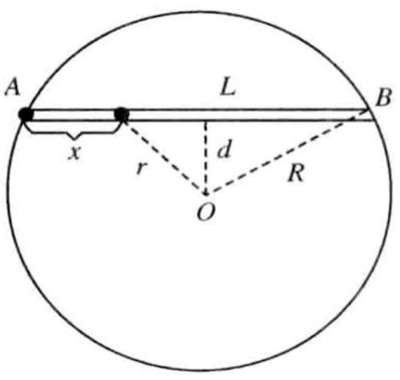
\includegraphics[width=0.3\linewidth,height=0.6\textheight,keepaspectratio]{figures/力图3-11-1.png}\\[2pt]
\textit{力图3-11-1}
\end{tabular}
\end{center}
\vfill
\newpage

\textbf{3-12} 如力图3-12-1，两个质量均为 $m$ 的小球串在质量可忽略的光滑细杆上，用两根完全相同的弹簧相连，两弹簧的劲度系数均为 $k$，原长均为 $l_{0}$，左侧弹簧的左端固定在细杆的 $O$ 点，细杆绕 $O$ 点在水平面内转动。


\begin{center}
\begin{tabular}{c}
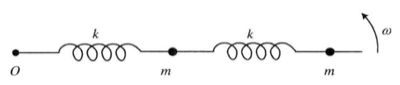
\includegraphics[width=0.3\linewidth,height=0.6\textheight,keepaspectratio]{figures/力图3-12-1.png}\\[2pt]
\textit{力图3-12-1}
\end{tabular}
\end{center}
\vfill
\newpage

\textbf{3-13} 如力图3-13-1，半径为 $R$ 的光滑圆环绕竖直的直径轴以角速度 $\omega$ 旋转。一质量为 $m$ 的小球串在圆环上，可沿环无摩擦地滑动。试求小球的平衡位置，并讨论平衡的稳定性。


\begin{center}
\begin{tabular}{c}
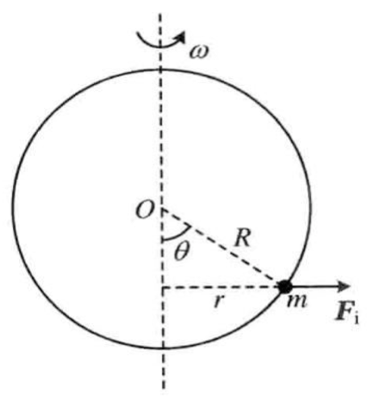
\includegraphics[width=0.3\linewidth,height=0.6\textheight,keepaspectratio]{figures/力图3-13-1.png}\\[2pt]
\textit{力图3-13-1}
\end{tabular}
\end{center}
\vfill
\newpage

\textbf{3-14} 如力图3-14-1，在相距为 $l$ 的两平行弹性墙壁之间，有质量为 $m$ 的弹性小球以垂直于壁的初速度 $v_{0}$ 往返弹跳，设壁的质量远大于 $m$，碰撞是完全弹性的，重力及空气阻力可略。

试求：1. 每壁所受的平均作用力。2. 若用外力使左壁以速度 $V$ $(V \ll v_{0})$ 缓缓右移，证明外力作功等于小球动能的增加。


\begin{center}
\begin{tabular}{c}
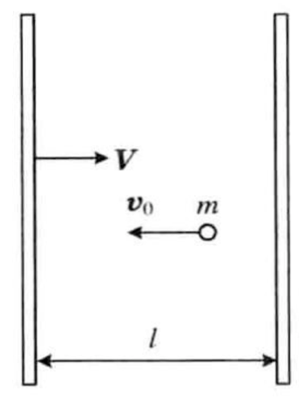
\includegraphics[width=0.3\linewidth,height=0.6\textheight,keepaspectratio]{figures/力图3-14-1.png}\\[2pt]
\textit{力图3-14-1}
\end{tabular}
\end{center}
\vfill
\newpage

\textbf{3-15} 如力图3-15-1，$A$、$B$、$C$ 三质点静止放置在光滑水平面上，它们的质量分别为 $m_{1}$、$m_{2}$、$m_{3}$，用柔软、不可伸长、质量可略的绳子相连并拉直，$AB$ 与 $BC$ 的夹角为 $\alpha$。以沿 $BC$ 方向的冲量 $I$ 作用于 $C$，试求质点 $A$ 开始运动时的初速。



\begin{center}
\begin{tabular}{c}
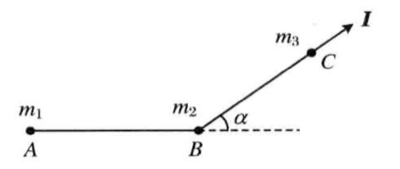
\includegraphics[width=0.3\linewidth,height=0.6\textheight,keepaspectratio]{figures/力图3-15-1.png}\\[2pt]
\textit{力图3-15-1}
\end{tabular}
\end{center}
\vfill
\newpage

\textbf{3-16} 如力图3-16-1，从地面发射的炮弹在达到最高点处炸裂为质量相等的两块。第一块在炸裂后沿原方向运动，第二块则沿水平方向被弹出。已知炮弹发射的初速为 $v_0$，发射角为 $\theta$。忽略空气阻力，炸裂后第二块的落地点距发射点的水平距离为 $S_1$。试求第一块落地点距发射点的水平距离 $S_2$。



\begin{center}
\begin{tabular}{c}
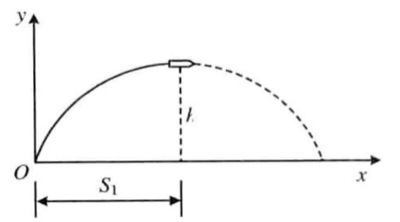
\includegraphics[width=0.3\linewidth,height=0.6\textheight,keepaspectratio]{figures/力图3-16-1.png}\\[2pt]
\textit{力图3-16-1}
\end{tabular}
\end{center}
\vfill
\newpage

\textbf{3-17} 地面上静止放置着质量为 $M$ 的平板车，车上有 $N$ 个人，每个人的质量均为 $m$。每个人以相同的相对速度 $u$（相对跳后的车速）沿水平方向从车后跳离平板车。忽略一切阻力。试问，在 $N$ 个人同时跳出和逐个跳出两种情况下，平板车在哪种情况下获得的动能大。
\vfill
\newpage

\textbf{3-18} 如力图3-18-1，地面上有质量为 $M$、倾角为 $\theta$ 的斜面体，其顶端高 $h$ 处有质量为 $m$ 的小木块。开始时两者均静止，然后小木块从斜面体顶端滑至底部。忽略各种摩擦及阻力。试求：以地面为参考系，在小木块下滑过程中斜面体的支持力对它所作的功。



\begin{center}
\begin{tabular}{c}
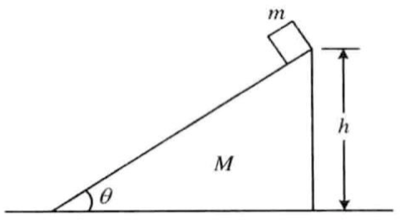
\includegraphics[width=0.3\linewidth,height=0.6\textheight,keepaspectratio]{figures/力图3-18-1.png}\\[2pt]
\textit{力图3-18-1}
\end{tabular}
\end{center}
\vfill
\newpage

\textbf{3-19} 如力图3-19-1，地面上静止地放置着质量为 $M$ 的木块，其底部为平面，上部有截面为半圆的凹槽，半径为 $R$，质量为 $m$ 的小球从最高处静止下滑。设各种摩擦及阻力均可略。试求：1. 在小球 $m$ 下滑过程中，$m$ 的绝对速度 $v$、$M$ 的绝对速度 $v_{M}$ 以及 $m$ 的相对速度 $v^{\prime}$ 随小球位置 $\theta$ 的变化规律。2. 小球 $m$ 在最低点时给木块 $M$ 的压力。



\begin{center}
\begin{tabular}{c}
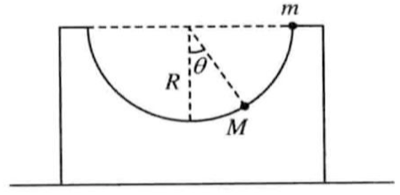
\includegraphics[width=0.3\linewidth,height=0.6\textheight,keepaspectratio]{figures/力图3-19-1.png}\\[2pt]
\textit{力图3-19-1}
\end{tabular}
\end{center}
\vfill
\newpage

\textbf{3-20} 如力图3-20-1，质量为 $m_{3}$ 的木块平放在地面上，通过劲度系数为 $k$ 的竖直弹簧与质量为 $m_{2}$ 的木块相联，达到平衡。质量为 $m_{1}$ 的小球从距 $m_{2}$ 为 $h$ 的高处静止下落，与 $m_{2}$ 作完全非弹性碰撞。试问：为使 $m_{2}$ 向上反弹时能带动 $m_{3}$ 刚好离开地面，$h$ 应为多少？



\begin{center}
\begin{tabular}{c}
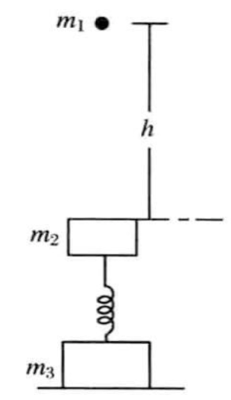
\includegraphics[width=0.3\linewidth,height=0.6\textheight,keepaspectratio]{figures/力图3-20-1.png}\\[2pt]
\textit{力图3-20-1}
\end{tabular}
\end{center}
\vfill
\newpage

\textbf{3-21} 如力图3-21-1所示，质量为 $M$ 的长滑块静止地放在光滑的水平桌面上，一质量可略的弹簧固定在滑块左端，弹簧的劲度系数为 $k$，滑块右端用一不可伸长的细绳固定在竖直墙上，细绳能承受的最大拉力为 $T_{0}$。一质量为 $m$，初速为 $v_{0}$（其方向水平向左）的小物在滑块上无摩擦地向左滑动，最终与弹簧相碰并压缩弹簧。


\begin{center}
\begin{tabular}{c}
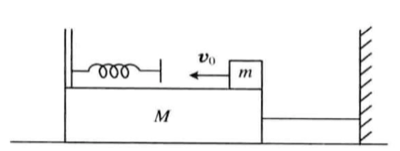
\includegraphics[width=0.3\linewidth,height=0.6\textheight,keepaspectratio]{figures/力图3-21-1.png}\\[2pt]
\textit{力图3-21-1}
\end{tabular}
\end{center}
\vfill
\newpage

\textbf{3-22} 如力图3-22-1，球1和球2的质量分别为 $m_{1}$ 和 $m_{2}$，放置在光滑水平地面上，球1以一定的水平初速 $v_{10}$ 向右沿两球连心线运动，球2则静止。两球连心线右侧有一竖直弹性墙。设两球之间以及球与墙之间的所有碰撞均为完全弹性碰撞。为了使两球能发生、而且只能发生两次碰撞，试问两球的质量之比 $\dfrac{m_1}{m_2}$ 应满足什么条件？


\begin{center}
\begin{tabular}{c}
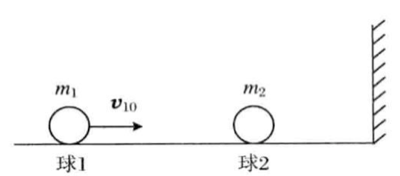
\includegraphics[width=0.3\linewidth,height=0.6\textheight,keepaspectratio]{figures/力图3-22-1.png}\\[2pt]
\textit{力图3-22-1}
\end{tabular}
\end{center}
\vfill
\newpage

\textbf{3-23} 如力图3-23-1，两根长度均为 $l$ 的刚性细杆，一端用质量为 $m$ 的球形铰链相连，两杆另一端分别安装质量为 $m$ 和 $2m$ 的小球。开始时两杆并拢，铰链球朝上，竖直放置在光滑桌面上，从静止释放，下面两球开始向两边滑动，两杆始终保持在同一铅垂面内。设三球本身的大小、轻杆的质量以及各种摩擦均可忽略。



\begin{center}
\begin{tabular}{c}
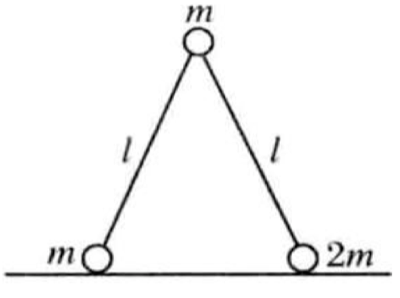
\includegraphics[width=0.3\linewidth,height=0.6\textheight,keepaspectratio]{figures/力图3-23-1.png}\\[2pt]
\textit{力图3-23-1}
\end{tabular}
\end{center}
\vfill
\newpage

\textbf{3-24} 小球从高度为 $h$ 处静止下落，与地面碰撞时的恢复系数为 $e$。忽略空气阻力，忽略碰撞过程所需时间。

\begin{center}
\begin{tabular}{c}
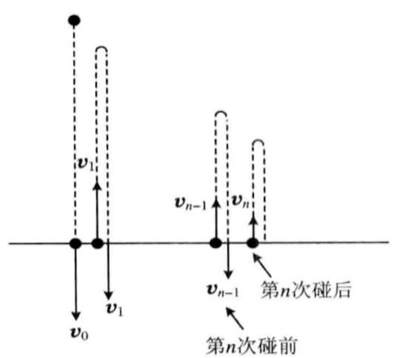
\includegraphics[width=0.3\linewidth,height=0.6\textheight,keepaspectratio]{figures/力图3-24-1.png}\\[2pt]
\textit{力图3-24-1}
\end{tabular}
\end{center}
\vfill
\newpage

\textbf{3-25} 如力图3-25-1，台阶每级的宽和高均为 $l$。一小球向下逐级弹跳，每次反弹后，相对本级达到的最高高度均为 $H$，每次的下落点均在各级的同一地点。已知小球与台阶碰撞时的恢复系数为 $e$，忽略空气阻力。



\begin{center}
\begin{tabular}{c}
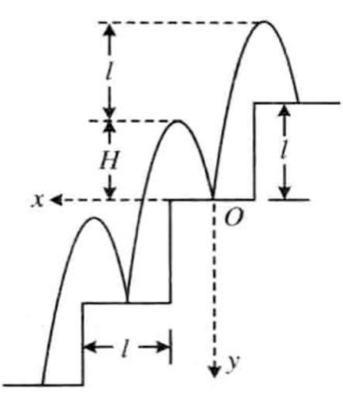
\includegraphics[width=0.3\linewidth,height=0.6\textheight,keepaspectratio]{figures/力图3-25-1.png}\\[2pt]
\textit{力图3-25-1}
\end{tabular}
\end{center}
\vfill
\newpage

\textbf{3-26} 如力图3-26-1，在固定斜面的 $O$ 点上方 $h = 1.60\,\mathrm{m}$ 处有一小球从静止自由下落。已知斜面是光滑的，倾角为 $\theta = 15^{\circ}$，小球与斜面碰撞时的恢复系数为 $e = 0.60$，忽略空气阻力。

试求：1. 小球碰后达到的最高点与 O 点之间的高度差 $h_{\max}$。2. 设小球碰后落在斜面上 P 点，则 O 点与 P 点的距离 $S$ 是多少？3. 小球与斜面碰撞后，其机械能损失的百分数是多少？



\begin{center}
\begin{tabular}{c}
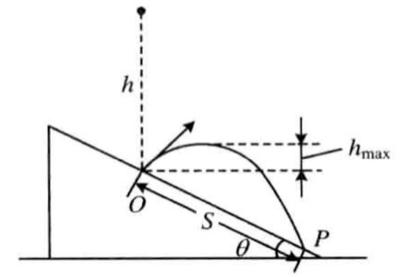
\includegraphics[width=0.3\linewidth,height=0.6\textheight,keepaspectratio]{figures/力图3-26-1.png}\\[2pt]
\textit{力图3-26-1}
\end{tabular}
\end{center}
\vfill
\newpage

\textbf{3-27} 如力图3-27-1，质量为 $M$ 的斜面体静止放置在光滑的水平桌面上，斜面体的倾角 $\theta = 15^{\circ}$。质量为 $m$ 的小球由静止自由下落到斜面体上，下落高度 $h = 1.60\,\mathrm{m}$。设斜面体表面是光滑的，并知小球碰后和碰前相对斜面体的相对速度在垂直于斜面方向的分量之比为 $e = 0.60$，碰撞点离桌面高度 $H = 1.00\,\mathrm{m}$，$M = 2m$。


\begin{center}
\begin{tabular}{c}
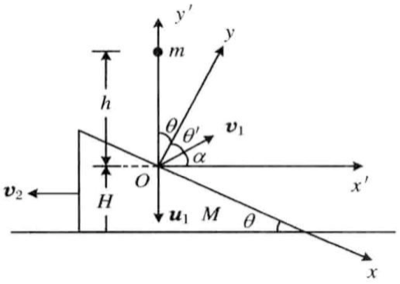
\includegraphics[width=0.3\linewidth,height=0.6\textheight,keepaspectratio]{figures/力图3-27-1.png}\\[2pt]
\textit{力图3-27-1}
\end{tabular}
\end{center}
\vfill
\newpage

\textbf{3-28} 一平板放置在光滑水平桌面上，一小球在此桌面上运动并与平板作完全弹性碰撞，设小球也是光滑的。试证明：不论平板原来静止或处于运动状态，相对平板而言，小球总是遵守入射角等于反射角的规律。
\vfill
\newpage

\textbf{3-29} 如图3-29-1，均匀圆环静止放置在光滑水平桌面上，圆环质量为 $M$，半径为 $R$。一质量为 $m$ 的质点以速度 $v_0$ 沿圆环的直径方向射向圆环，碰撞是完全弹性的。试求碰后圆环的运动状态和质点的运动状态。


\begin{center}
\begin{tabular}{c}
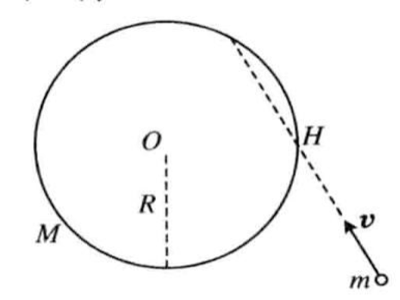
\includegraphics[width=0.3\linewidth,height=0.6\textheight,keepaspectratio]{figures/力图3-29-1.png}\\[2pt]
\textit{力图3-29-1}
\end{tabular}
\end{center}
\vfill
\newpage

\textbf{3-30} 三质点的质量分别为 $m_{1}$、$m_{2}$、$m_{3}$，以万有引力相互作用，绕垂直于三质点所在平面并通过质心 C 的转轴旋转。

试问：为使三质点的相对位置保持不变，需满足什么条件？
\vfill
\newpage

\textbf{3-31} 质量为 $M$ 的平板车静止在光滑地面上，车上有 $N$ 个人，每人的质量均为 $m$，若每人消耗同样的体力（即每人作功相同）沿水平方向向后跳，忽略空气阻力，人可看作是质点。
\vfill
\newpage

\textbf{3-32} 如力图3-32-1，质量分别为 $m_{1}$ 和 $m_{2}$ 的两木块用劲度系数为 $k$ 的弹簧相连，静止地放在光滑地面上。质量为 $m$ 的子弹以水平初速 $v_{0}$ 射入木块 $m_{1}$，设子弹射入过程的时间极短。


\begin{center}
\begin{tabular}{c}
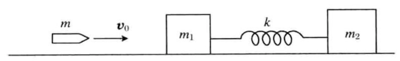
\includegraphics[width=0.3\linewidth,height=0.6\textheight,keepaspectratio]{figures/力图3-32-1.png}\\[2pt]
\textit{力图3-32-1}
\end{tabular}
\end{center}
\vfill
\newpage

\textbf{3-33} 如力图3-33-1，在光滑地面上静止地放着质量为 $m$ 的箱子。在箱内光滑的底面上，质量也为 $m$ 的滑块以水平初速 $v_{0}$ 开始运动，并与两壁反复碰撞。已知滑块与箱子每碰一次后，两者的相对速度改变 $e = \sqrt[4]{\frac{1}{2}}$ 倍。

试求：1. 最多经几次碰撞后，系统总能量的损耗不大于40\%。2. 从滑块开始运动到完成上述次数的碰撞后，箱子的平均速度是多少？


\begin{center}
\begin{tabular}{c}
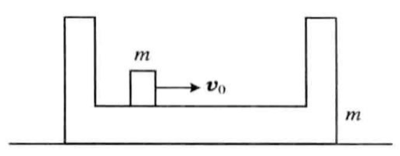
\includegraphics[width=0.3\linewidth,height=0.6\textheight,keepaspectratio]{figures/力图3-33-1.png}\\[2pt]
\textit{力图3-33-1}
\end{tabular}
\end{center}
\vfill
\newpage

\textbf{3-34} 动能为 $E_0$ 的 ${}^4\mathrm{He}$ 核轰击静止的 ${}^7\mathrm{Li}$ 核，作完全非弹性碰撞后成为复合核 ${}^{11}\mathrm{B}$，${}^{11}\mathrm{B}$ 进一步分裂为 ${}^{10}\mathrm{B}$ 和中子 ${}^1\mathrm{n}$。上述核反应过程需消耗能量 $Q = 2.8\,\mathrm{MeV}$。反应方程为
\[
{}^4\mathrm{He} + {}^{7}\mathrm{Li} \rightarrow ({}^{11}\mathrm{B}) \rightarrow {}^{10}\mathrm{B} + {}^{1}\mathrm{n} - 2.8\,\mathrm{MeV}
\]

试求：上述核反应过程所需的 $E_{0}$ 的最小值是多少？相应的中子动能为多大？
\vfill
\newpage

\textbf{3-35} 一物体作直线运动，其质量不断随时间变化。设该物体在 $t$ 时刻的质量为 $M(t)$，速度为 $v(t)$。试证明下述密舍尔斯基方程：
\[
M\frac{\mathrm{d}v}{\mathrm{d}t} = (u - v)\frac{\mathrm{d}M}{\mathrm{d}t} + F
\]

式中 $F$ 是质量不断变化的主体所受的合外力，$u$ 是附加物附加到主体前的绝对速度或抛出物抛离主体后的绝对速度。
\vfill
\newpage

\textbf{3-36} 竖直下垂的绳子从静止自由下落，开始时绳下端刚好与地面接触。设绳均匀柔软，全长为 $l$。

试证明：下落过程中地面所受压力等于已经落在地面上的绳子重量的3倍。
\vfill
\newpage

\textbf{3-37} 火箭从地面竖直向上发射。已知火箭自身质量为 $M_{s}$，燃料的初始质量为 $M_{f}$，燃气相对火箭的喷射速度为 $v^{\prime}$，单位时间的喷气质量为 $a$。设在火箭上升的高度范围内 $g$ 为常量，忽略空气阻力。

试求：1. 火箭的推力和加速度。2. 任意时刻火箭的速度和上升高度。3. 燃料耗尽时，火箭的加速度、速度和高度。4. 火箭能达到的最大高度及所需时间。
\vfill
\newpage

\textbf{3-38} 如力图3-38-1，质量为 $m$ 的小球下系一条足够长的柔软均匀且不可伸长的绳子。绳子的质量线密度为 $\lambda$。将小球以初速 $v_{0}$ 从地面竖直上抛，忽略空气阻力。

试问：在上升过程中，小球的速率怎样随高度变化？


\begin{center}
\begin{tabular}{c}
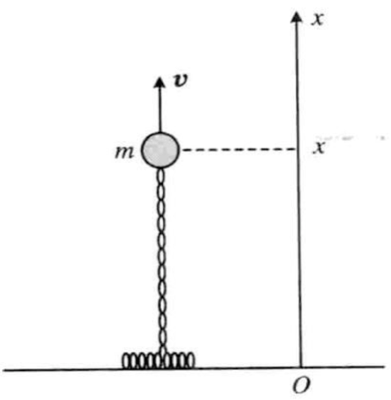
\includegraphics[width=0.3\linewidth,height=0.6\textheight,keepaspectratio]{figures/力图3-38-1.png}\\[2pt]
\textit{力图3-38-1}
\end{tabular}
\end{center}
\vfill
\newpage

\textbf{3-39} 球状小水滴在静止的雾气中下落，下落过程中吸附了全部所遇到的水分子。设水滴始终保持球状，设雾气密度均匀，忽略空气的粘滞力，重力加速度取恒定值 $g$。

试证明经过足够长时间后，水滴加速度趋于稳定值，并求出此稳定值。
\vfill


\chapter{角动量、有心运动}
\textbf{4-1} 试根据牛顿万有引力定律证明开普勒行星运动三定律。
\vfill
\newpage

\textbf{4-2} 已知行星绕太阳沿椭圆轨道运动（开普勒第一定律）。试证明行星所受太阳引力必定与距离平方成反比。
\vfill
\newpage

\textbf{4-3} 如力图4-3-1，设质量为 $M$ 的恒星固定不动。质量为 $m$ 的行星在其引力作用下运动，运动轨迹可以是椭圆、抛物线或双曲线。试求各种轨迹相应的总能量，并给出各种轨迹的判据。



\begin{center}
\begin{tabular}{c}
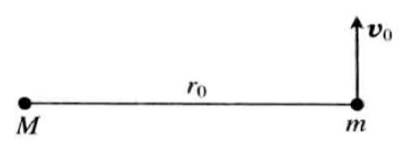
\includegraphics[width=0.3\linewidth,height=0.6\textheight,keepaspectratio]{figures/力图4-3-1.png}\\[2pt]
\textit{力图4-3-1}
\end{tabular}
\end{center}
\vfill
\newpage

\textbf{4-4} 空间两质点的质量分别为 $m_{1}$ 和 $m_{2}$，彼此以万有引力相互作用。开始时两质点静止，相距 $r_0$，在引力作用下彼此接近并相碰。试求两质点从开始运动到相碰所经历的时间。
\vfill
\newpage

\textbf{4-5} 如力图4-5-1所示，质量为 $m = 1.20 \times 10^{4}\,\mathrm{kg}$ 的飞船在离月球表面高度为 $h = 100\,\mathrm{km}$ 处绕月球作圆周运动。飞船采用两种登月方式。1. 在 A 点向前（即向力图4-5-1上方）短时间喷气，使飞船与月球相切地到达月球上的 B 点（AB 通过月球中心 O 点）。2. 在 A 点向外侧（即向力图4-5-1右方）沿月球半径短时间喷气，使飞船与月球相切地到达月球上的 C 点（CO 与 AB 垂直）。设喷气相对飞船的速度为 $u = 1.00 \times 10^{4}\,\mathrm{m/s}$。已知月球半径 $R = 1700\,\mathrm{km}$，月球重力加速度（当作常量）$g = 1.700\,\mathrm{m/s^2}$。试求：两种登月方式各需的燃料质量。



\begin{center}
\begin{tabular}{c}
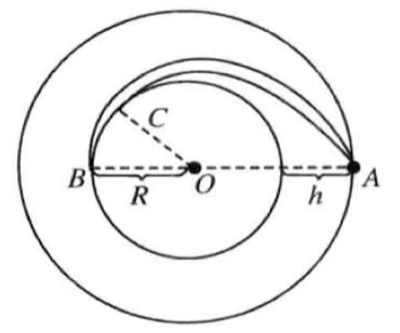
\includegraphics[width=0.3\linewidth,height=0.6\textheight,keepaspectratio]{figures/力图4-5-1.png}\\[2pt]
\textit{力图4-5-1}
\end{tabular}
\end{center}
\vfill
\newpage

\textbf{4-6} 如力图4-6-1，飞船绕地球作圆周运动，离地面的高度 $h = 800\,\mathrm{km}$，地球半径 $R = 6.40 \times 10^{3}\,\mathrm{km}$，飞船圆轨道半径 $r_{0} = R + h$，飞船速度 $v_{0} = 3.00 \times 10^{4}\,\mathrm{km/h}$。经过短暂的沿矢径向外侧喷气，飞船获得了指向地心 $O$ 的附加速度 $v_{r} = 800\,\mathrm{km/h}$，其轨道变为椭圆。设喷气后飞船的质量可看作不变。试求：飞船椭圆轨道的近地点和远地点离地面的高度。


\begin{center}
\begin{tabular}{c}
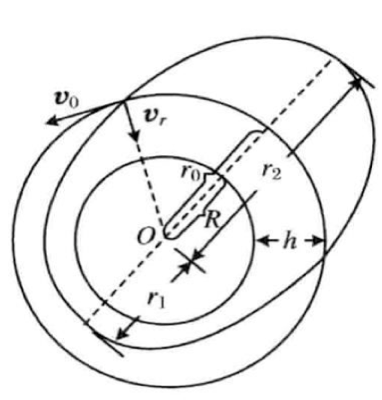
\includegraphics[width=0.3\linewidth,height=0.6\textheight,keepaspectratio]{figures/力图4-6-1.png}\\[2pt]
\textit{力图4-6-1}
\end{tabular}
\end{center}
\vfill
\newpage

\textbf{4-7} 如力图4-7-1，飞船总质量为 $m$，内装质量为 $m_0$ 的探测器，绕地球沿椭圆轨道运行，近地点与地心距离为 $r_1$，速度为
\[
v_{1} = \sqrt{\frac{2\alpha GM}{r_1}}
\]

1. 试证明 $1 > \alpha > \dfrac{1}{2}$。

2. 如力图4-7-2，飞船在近地点向前发射探测器，并使探测器沿抛物线轨道运动。发射后，飞船沿圆轨道运行。试求：质量比 $\dfrac{m_0}{m}$ 及发射探测器的相对速度 $u$。

3. 如力图4-7-3，若在远地点以上述相对速度 $u$ 发射探测器，试求探测器运行的轨道。



\begin{center}
\begin{tabular}{c}
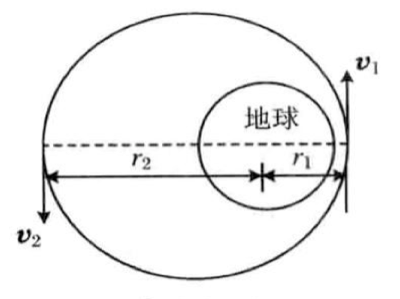
\includegraphics[width=0.3\linewidth,height=0.6\textheight,keepaspectratio]{figures/力图4-7-1.png}\\[2pt]
\textit{力图4-7-1}
\end{tabular}
\qquad
\begin{tabular}{c}
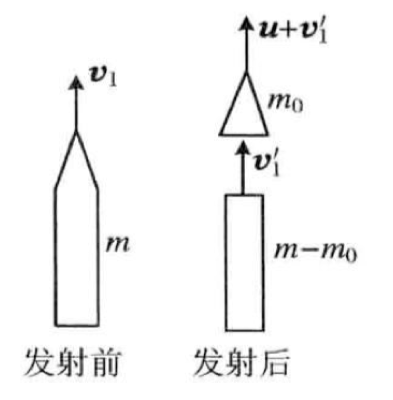
\includegraphics[width=0.3\linewidth,height=0.6\textheight,keepaspectratio]{figures/力图4-7-2.png}\\[2pt]
\textit{力图4-7-2}
\end{tabular}
\qquad
\begin{tabular}{c}
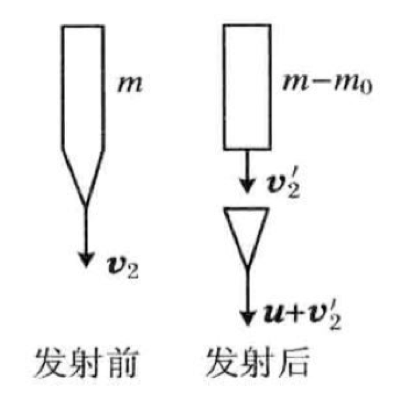
\includegraphics[width=0.3\linewidth,height=0.6\textheight,keepaspectratio]{figures/力图4-7-3.png}\\[2pt]
\textit{力图4-7-3}
\end{tabular}
\end{center}
\vfill
\newpage

\textbf{4-8} 如力图4-8-1，地球沿半径为 $R_0$ 的圆轨道绕太阳运动。彗星绕太阳沿抛物线运动。已知抛物线与地球圆轨道一直径的两端相交。忽略地球与彗星之间的引力。

试求：1. 彗星抛物线轨道的方程。2. 彗星的最大速率是地球公转速率的几倍？3. 彗星在地球轨道内的运行时间是多少地球年？


\begin{center}
\begin{tabular}{c}
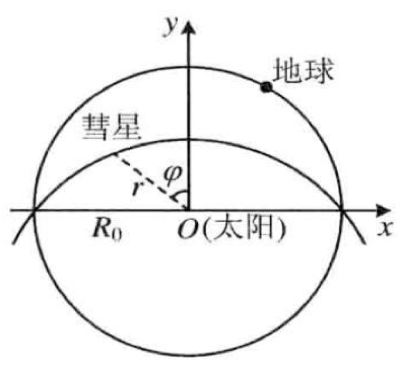
\includegraphics[width=0.3\linewidth,height=0.6\textheight,keepaspectratio]{figures/力图4-8-1.png}\\[2pt]
\textit{力图4-8-1}
\end{tabular}
\end{center}
\vfill
\newpage

\textbf{4-9} 如力图4-9-1，质量为 $M$ 的宇航站和与其对接上的质量为 $m$ 的飞船一起绕地球沿圆轨道运动，轨道半径是地球半径 $R$ 的 $n$ 倍，$n = 1.25$。某一瞬时，宇航站将飞船沿运动方向发射出去。发射后，飞船和宇航站将分别沿各自新的椭圆轨道运行。已知飞船椭圆轨道的远地点离地球中心的距离为 $8nR$。设发射飞船后宇航站的质量不变（即忽略喷气的质量）。

试问：当质量比 $\dfrac{m}{M}$ 为何值时，飞船绕地球一周后刚好与宇航站相遇。


\begin{center}
\begin{tabular}{c}
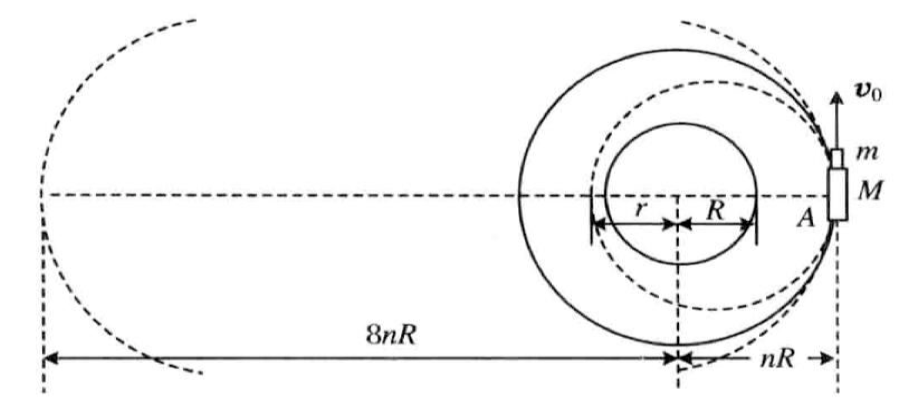
\includegraphics[width=0.3\linewidth,height=0.6\textheight,keepaspectratio]{figures/力图4-9-1.png}\\[2pt]
\textit{力图4-9-1}
\end{tabular}
\end{center}
\vfill
\newpage

\textbf{4-10} 如力图4-10-1，从地球发射火箭到火星进行探测，发射后火箭绕太阳沿椭圆轨道运行。为了节省能量，火箭离开地球的速度方向与地球绕太阳公转的速度方向一致，并且选择适当的发射时机，使火箭椭圆轨道的远日点为火星，近日点为地球。假定地球和火星均绕太阳作圆周运动，圆轨道半径分别为 $r_{\text{地}}$ 和 $r_{\text{火}}$，忽略其他行星对火箭的引力作用。

试问：1. 火箭应以多大的相对速度离开地球？2. 火箭到达火星要用多长时间？


\begin{center}
\begin{tabular}{c}
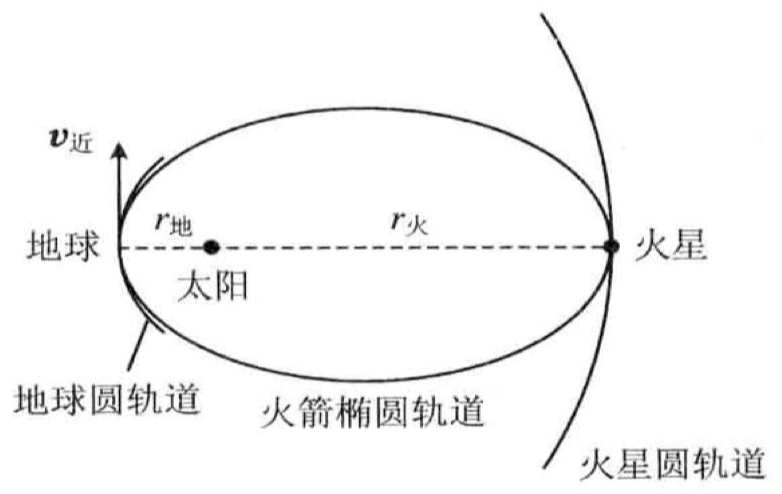
\includegraphics[width=0.3\linewidth,height=0.6\textheight,keepaspectratio]{figures/力图4-10-1.png}\\[2pt]
\textit{力图4-10-1}
\end{tabular}
\end{center}
\vfill
\newpage

\textbf{4-11} 如力图4-11-1，宇宙飞船绕火星沿圆轨道运行，运动速度为 $v_{0}$。已知火星半径为 $R$，飞船圆轨道离火星表面的高度为 $H$。今飞船在极短时间内，沿圆轨道径向向外侧点火喷气，使飞船获得指向火星的径向速度 $\alpha v_{0}$，$\alpha$ 是远小于1的常数。因喷气量很小，喷气后飞船的质量可视为不变。喷气后，飞船绕火星沿新的椭圆轨道运行。

试求：1. 飞船椭圆轨道近火星点距火星表面的高度 $h_{A}$ 以及远火星点距火星表面的高度 $h_{B}$。2. 飞船绕椭圆轨道的运行周期。


\begin{center}
\begin{tabular}{c}
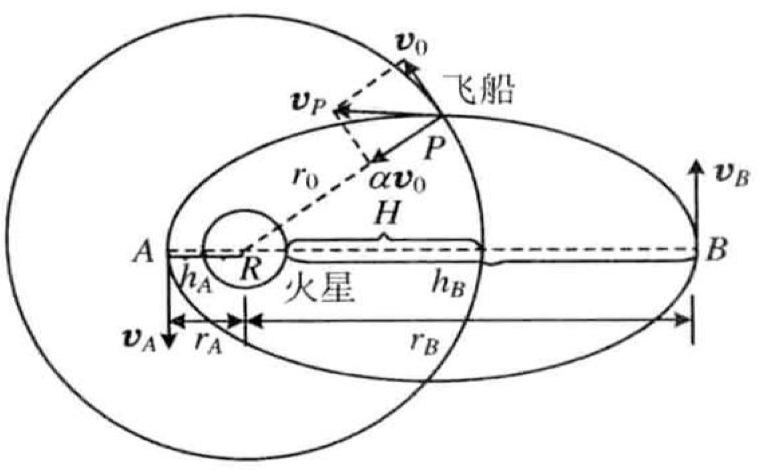
\includegraphics[width=0.3\linewidth,height=0.6\textheight,keepaspectratio]{figures/力图4-11-1.png}\\[2pt]
\textit{力图4-11-1}
\end{tabular}
\end{center}
\vfill
\newpage

\textbf{4-12} 将宇宙飞船从地面发射到太阳系外，有两个方案。方案一：以足够大的速度（大于太阳系逃逸速度）直接发射。方案二：使宇宙飞船接近太阳系的一个外层行星（例如火星），在它的作用下，改变运动方向，然后逃离太阳系。

试求：1. 按方案一，确定从地面发射飞船所必需的相对地球的最小速度 $v_{a}$ 及发射方向。2. 按本题第1问的方向相对地球以 $v_{b}$ 从地面发射飞船，求飞船穿过火星轨道的速度，即求飞船速度在火星轨道的切线分量和垂直分量。设飞船穿过火星轨道时，火星离飞船很远。3. 使飞船进入火星引力场，但仍可飞出太阳系，求从地面发射的速度。设飞船相对地球的发射方向与本题第一问相同，设飞船沿火星轨道的切线方向脱离火星引力场。4. 估计方案二比方案一节省能量的最大百分比。

设所有行星在同一平面内以同一方向绕太阳在圆轨道上运行。设空气阻力及地球自转的影响均可忽略。

数据：地球绕太阳公转的速度为 $30\,\mathrm{km/s}$，地球到太阳的距离与火星到太阳的距离之比为 $2{:}3$，地球半径 $R_E = 6400\,\mathrm{km}$，地球表面的重力加速度 $g = 9.80\,\mathrm{m/s^2}$。
\vfill
\newpage

\textbf{4-13} 如力图4-13-1，劲度系数 $k = 3$ 的弹簧一端 $O$ 固定，另一端有质量 $m = 20\,\mathrm{g}$ 的质点。质点绕 $O$ 点在光滑水平面内作匀速圆周运动，总机械能为 $E_0 = 12\,\mathrm{J}$。突然沿径向给质点一击，使之获得沿径向向外的速度 $v_{r0} = 1.0\,\mathrm{m/s}$。设弹簧的原长很小，可忽略不计。

1. 试用能量曲线 $(E \sim r)$ 描述质点受打击前、后的运动状态。2. 试求质点运动的半径范围。



\begin{center}
\begin{tabular}{c}
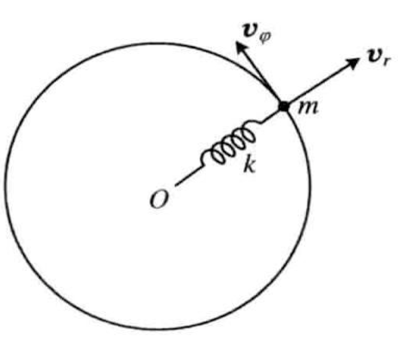
\includegraphics[width=0.3\linewidth,height=0.6\textheight,keepaspectratio]{figures/力图4-13-1.png}\\[2pt]
\textit{力图4-13-1}
\end{tabular}
\end{center}
\vfill
\newpage

\textbf{4-14} 一质量为 $m$ 的行星绕质量为 $M$ 的恒星运动。设在行星与恒星之间的整个空间内均匀分布着稀薄的宇宙尘埃，已知尘埃的密度为 $\rho$ 且很小，可以忽略行星与尘埃之间的直接碰撞作用。

1. 试问，对于角动量为 $L$ 的圆形行星轨道，其半径 $r_0$ 应满足什么方程（列出方程即可，不必求解）？

2. 考虑相对上述圆轨道稍有偏离的另一轨道，试解释它是一条作进动的椭圆轨道，进动方向与行星运行方向相反，并求出进动的角速度。
\vfill


\chapter{静力平衡}
\textbf{5-1} 如力图5-1-1，静止的圆锥体竖直放置，顶角为 $\alpha$。质量为 $m$ 且分布均匀的链条环水平地套在圆锥体上，忽略链条与圆锥体之间的摩擦力。试求链条中的张力。



\begin{center}
\begin{tabular}{c}
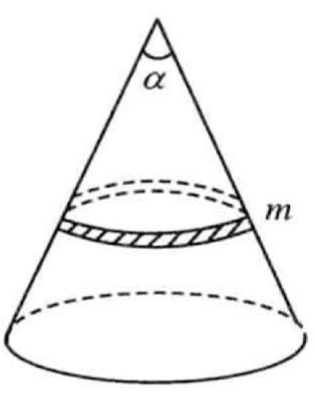
\includegraphics[width=0.3\linewidth,height=0.6\textheight,keepaspectratio]{figures/力图5-1-1.png}\\[2pt]
\textit{力图5-1-1}
\end{tabular}
\end{center}
\vfill
\newpage

\textbf{5-2} 如力图5-2-1，均匀杆 $AB$ 长 $l$，重 $w_0$，$A$ 端与粗糙的竖直墙接触，$B$ 端用不可伸长的绳悬挂于竖直墙的 $C$ 点，杆呈水平状态，绳与杆的夹角为 $\theta$。

试问：1. 为了使杆达到静力平衡，杆 A 端与竖直墙之间的摩擦系数 $\mu$ 应满足什么条件？2. 若在杆上悬挂另一重量为 $w = \dfrac{w_0}{2}$ 的重物，为了使杆仍维持平衡，所需摩擦系数的最小值与悬点的位置有何关系？



\begin{center}
\begin{tabular}{c}
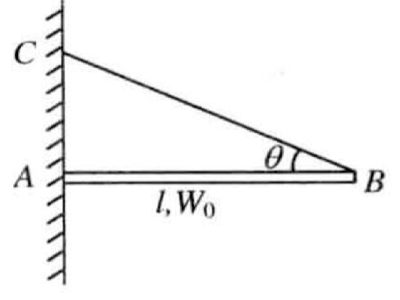
\includegraphics[width=0.3\linewidth,height=0.6\textheight,keepaspectratio]{figures/力图5-2-1.png}\\[2pt]
\textit{力图5-2-1}
\end{tabular}
\end{center}
\vfill
\newpage

\textbf{5-3} 如力图5-3-1，质量为 $m$、长为 $L$ 的均匀细直杆竖直放置，杆下端与地面之间的摩擦系数为 $\mu$，杆上端用绳索拉住，绳与直杆之间的夹角为 $\theta$。在离地面高度为 $h$ 处以水平力 $F$ 作用于直杆。试问为使直杆不滑倒，作用力 $F$ 的最大值应是多少？



\begin{center}
\begin{tabular}{c}
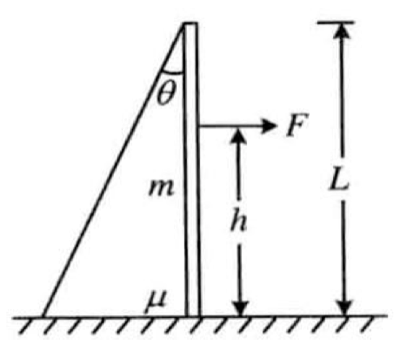
\includegraphics[width=0.3\linewidth,height=0.6\textheight,keepaspectratio]{figures/力图5-3-1.png}\\[2pt]
\textit{力图5-3-1}
\end{tabular}
\end{center}
\vfill
\newpage

\textbf{5-4} 如力图5-4-1，在半径为 $R$ 的光滑半球形凹面内，有一刚性均匀细杆达到平衡。已知杆在半球面内那部分的长度为 $l$。试求杆露出半球面外那部分的长度。


\begin{center}
\begin{tabular}{c}
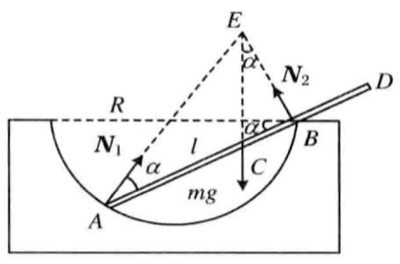
\includegraphics[width=0.3\linewidth,height=0.6\textheight,keepaspectratio]{figures/力图5-4-1.png}\\[2pt]
\textit{力图5-4-1}
\end{tabular}
\end{center}
\vfill
\newpage

\textbf{5-5} 如力图5-5-1，三个半径和质量均相同的圆柱体按图中的方式堆放在地面上，互相接触。已知圆柱体之间的摩擦系数为 $\mu_{1}$，圆柱体与地面之间的摩擦系数为 $\mu_{2}$。试求使三圆柱体达到平衡所需之 $\mu_{1}$ 和 $\mu_{2}$ 的下限值。



\begin{center}
\begin{tabular}{c}
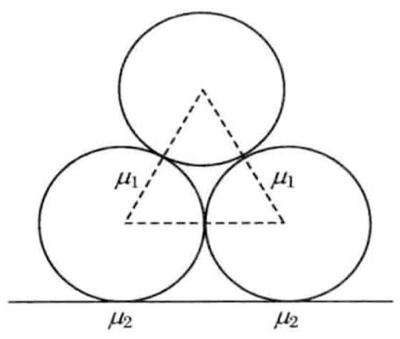
\includegraphics[width=0.3\linewidth,height=0.6\textheight,keepaspectratio]{figures/力图5-5-1.png}\\[2pt]
\textit{力图5-5-1}
\end{tabular}
\end{center}
\vfill
\newpage

\textbf{5-6} 如力图5-6-1所示，均匀木板 $AB$ 长 $L = 100\,\mathrm{cm}$，重 $2G$，一端用铰链固定于竖直墙，另一端用水平线拉住，木板与竖直墙之间的夹角为 $60^{\circ}$。三个完全相同的球按力图5-6-1中的位置放在木板上，球半径均为 $R = 10\,\mathrm{cm}$，重量均为 $G$。设球与墙，球与木板，球与球之间的摩擦力均可忽略。试求水平线的拉力 $T$。



\begin{center}
\begin{tabular}{c}
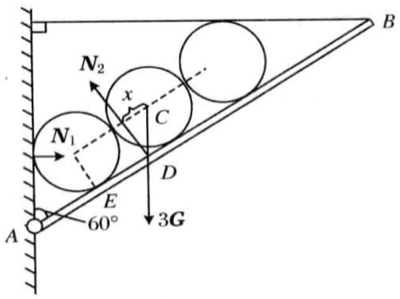
\includegraphics[width=0.3\linewidth,height=0.6\textheight,keepaspectratio]{figures/力图5-6-1.png}\\[2pt]
\textit{力图5-6-1}
\end{tabular}
\end{center}
\vfill
\newpage

\textbf{5-7} 如力图5-7-1所示，AB、BC、CD和DE为质量可略的等长细线，长度均为 $5\,\mathrm{m}$，$A$ 端和 $E$ 端悬挂在水平天花板上，$AE = 14\,\mathrm{m}$。B 和 D 是质量均为 $m_0 = 7\,\mathrm{kg}$ 的相同小球。质量为 $m$ 的重物挂于 $C$ 点，平衡时 $C$ 点离天花板的垂直距离为 $7\,\mathrm{m}$。

1. 试求质量 $m$。2. 今用外力将 $C$ 点缓慢提升，使BCD位于同一水平线上，试求此过程中外力作的功。



\begin{center}
\begin{tabular}{c}
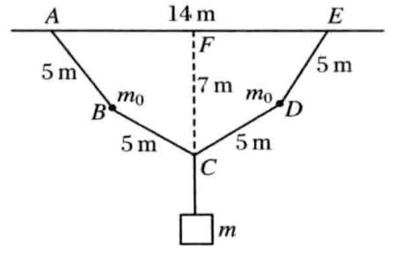
\includegraphics[width=0.3\linewidth,height=0.6\textheight,keepaspectratio]{figures/力图5-7-1.png}\\[2pt]
\textit{力图5-7-1}
\end{tabular}
\end{center}
\vfill
\newpage

\textbf{5-8} 如力图5-8-1所示，浮子由两个半径为 $R$ 的球冠相合而成，其质量为 $m_{1}$，中心厚度为 $h$ $(h < 2R)$。长为 $l$，质量为 $m_{2}$ 的均匀细杆从浮子中心垂直插入，下端刚好到达下球冠表面。细杆的铅垂位置显然是一个平衡位置。试分析平衡的稳定性。



\begin{center}
\begin{tabular}{c}
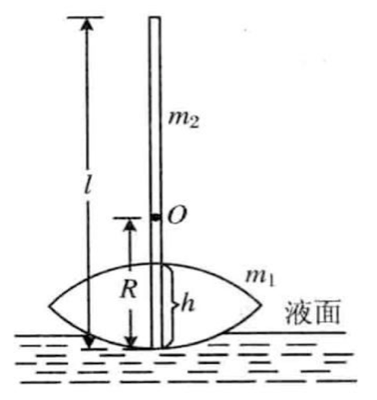
\includegraphics[width=0.3\linewidth,height=0.6\textheight,keepaspectratio]{figures/力图5-8-1.png}\\[2pt]
\textit{力图5-8-1}
\end{tabular}
\end{center}
\vfill
\newpage

\textbf{5-9} 如力图5-9-1，五根质量分布均匀、质量和长度完全相同的细杆，用光滑铰链互相连结并悬挂起来。试求平衡时由细杆组成的五边形的五个顶角。



\begin{center}
\begin{tabular}{c}
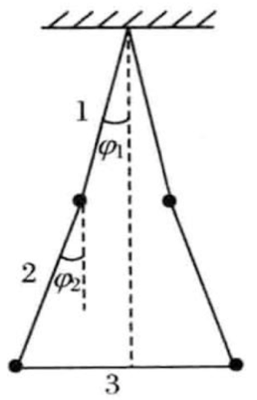
\includegraphics[width=0.3\linewidth,height=0.6\textheight,keepaspectratio]{figures/力图5-9-1.png}\\[2pt]
\textit{力图5-9-1}
\end{tabular}
\end{center}
\vfill
\newpage

\textbf{5-10} 如力图5-10-1，半径为 $R$ 的圆柱体在水平面上固定不动，厚度为 $t$ 的均匀木板水平地放置在圆柱体上，其长度方向（力图5-10-1中的横向）与圆柱体的轴（水平方向与力图5-10-1的平面垂直）垂直，并处于平衡状态。试问厚度 $t$ 取何值时属稳定平衡。



\begin{center}
\begin{tabular}{c}
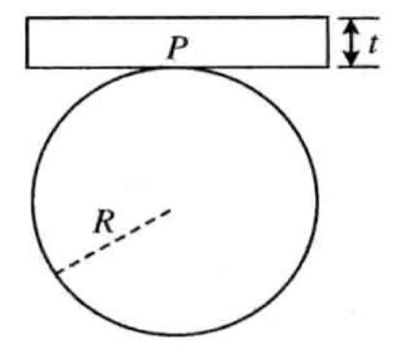
\includegraphics[width=0.3\linewidth,height=0.6\textheight,keepaspectratio]{figures/力图5-10-1.png}\\[2pt]
\textit{力图5-10-1}
\end{tabular}
\end{center}
\vfill
\newpage

\textbf{5-11} 如力图5-11-1，四根质量、长度都相同的均匀木条用光滑铰链连接成菱形，一均匀圆盘静止地夹在两木条之间，整个系统竖直悬挂起来，悬点为 $O$ 点。设圆盘与木条之间的接触是光滑的。已知每根木条的长度 $l = 50\,\mathrm{cm}$，质量 $m = 50\,\mathrm{g}$；圆盘的半径 $r = 8\,\mathrm{cm}$，质量 $M = 200\,\mathrm{g}$。试求系统的平衡位置（用 $\theta$ 角表示）。


\begin{center}
\begin{tabular}{c}
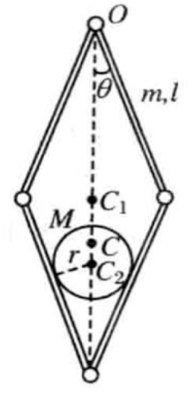
\includegraphics[width=0.3\linewidth,height=0.6\textheight,keepaspectratio]{figures/力图5-11-1.png}\\[2pt]
\textit{力图5-11-1}
\end{tabular}
\end{center}
\vfill
\newpage

\textbf{5-12} 如力图5-12-1，质量分布均匀的柔软细绳全长 $L$，质量线密度为 $\lambda$，悬挂在两根竖直杆上，测得细绳在两悬挂点的切线与竖直杆之间的夹角分别为 $\theta_{1}$ 和 $\theta_{2}$。

1. 试求细绳两端所受的拉力。2. 若左悬点的高度为 $H$，试导出在 $Oxy$ 坐标系中的悬链线方程。



\begin{center}
\begin{tabular}{c}
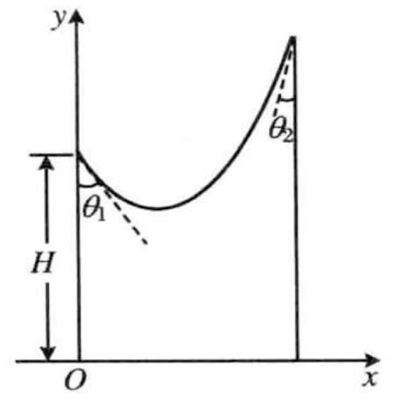
\includegraphics[width=0.3\linewidth,height=0.6\textheight,keepaspectratio]{figures/力图5-12-1.png}\\[2pt]
\textit{力图5-12-1}
\end{tabular}
\end{center}
\vfill


\chapter{刚体动力学}
\textbf{6-1} 汽车在后轮的推动下，以加速度 $a$ 在地面上沿直线前进。已知汽车前轮与后轮的间距为 $2l$，质心位于前后轮的中央，离地高度为 $h$，后轮与地面之间的摩擦系数为 $\mu$，前轮为非驱动轮，与地面的摩擦可略。试问：$\mu$ 至少为多大时，后轮不致打滑？



\begin{center}
\begin{tabular}{c}
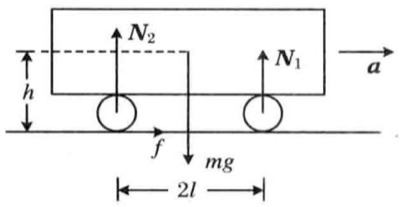
\includegraphics[width=0.3\linewidth,height=0.6\textheight,keepaspectratio]{figures/力图6-1-1.png}\\[2pt]
\textit{力图6-1-1}
\end{tabular}
\end{center}
\vfill
\newpage

\textbf{6-2} 如力图6-2-1，质量为 $m$ 的均匀圆柱体，截面半径为 $R$，长为 $2R$。试求：圆柱体绕通过质心及两底面边缘的转轴的转动惯量。



\begin{center}
\begin{tabular}{c}
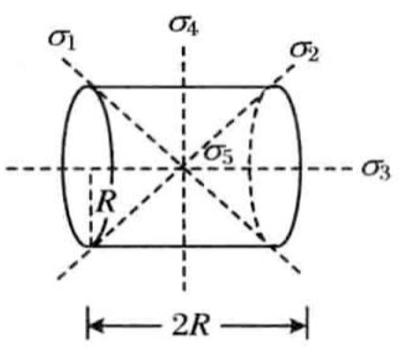
\includegraphics[width=0.3\linewidth,height=0.6\textheight,keepaspectratio]{figures/力图6-2-1.png}\\[2pt]
\textit{力图6-2-1}
\end{tabular}
\end{center}
\vfill
\newpage

\textbf{6-3} 如力图6-3-1，长为 $l$ 的均匀细杆水平地放置在桌面上，质心离桌边缘的距离为 $b$，从静止下落。已知杆与桌边缘之间的摩擦系数为 $\mu$。试求杆开始滑动时的角度 $\theta_C$。



\begin{center}
\begin{tabular}{c}
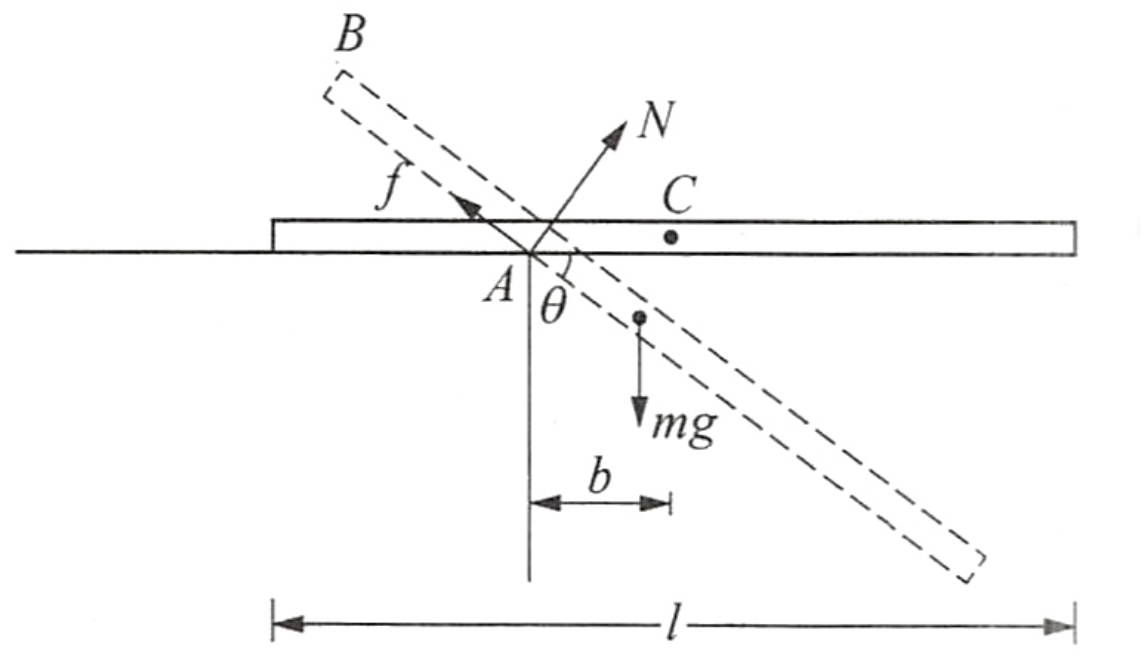
\includegraphics[width=0.3\linewidth,height=0.6\textheight,keepaspectratio]{figures/力图6-3-1.png}\\[2pt]
\textit{力图6-3-1}
\end{tabular}
\end{center}
\vfill
\newpage

\textbf{6-4} 如力图6-4-1，实心圆柱体从桌边由静止下滚，圆柱体与桌边之间的摩擦系数为 $\mu$。圆柱体下滚过程中所转过的角度用 $\theta$ 表示。试求圆柱体开始相对桌边滑动时相应角度 $\theta$ 所满足的关系式，并用图解法在图上标出这个角度以及不滑动的转角范围。



\begin{center}
\begin{tabular}{c}
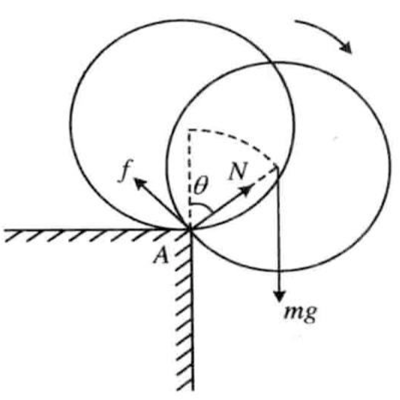
\includegraphics[width=0.3\linewidth,height=0.6\textheight,keepaspectratio]{figures/力图6-4-1.png}\\[2pt]
\textit{力图6-4-1}
\end{tabular}
\end{center}
\vfill
\newpage

\textbf{6-5} 如力图6-5-1，均匀细麦杆长 $l$，可绕通过中心 $O$ 的固定水平轴在铅垂面内自由转动。开始时麦杆静止于水平位置。一质量与麦杆相同的甲虫以速度 $v_{0}$ 垂直落到麦杆的 $\dfrac{1}{4}$ 长度处，落下后立即向端点爬行。

试问：1. 为使麦杆以均匀的角速度转动，甲虫沿麦杆爬行的速度应是多少？2. 甲虫轨迹的参变方程是什么？3. 为了使甲虫在麦杆转到铅直位置前能爬到端点，甲虫下落速度 $v_{0}$ 的最高值是多少？



\begin{center}
\begin{tabular}{c}
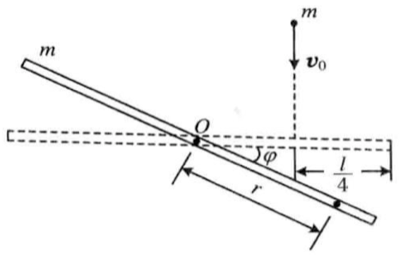
\includegraphics[width=0.3\linewidth,height=0.6\textheight,keepaspectratio]{figures/力图6-5-1.png}\\[2pt]
\textit{力图6-5-1}
\end{tabular}
\end{center}
\vfill
\newpage

\textbf{6-6} 如力图6-6-1，半径为 $R$ 的均匀实心圆柱体在水平地面上作纯滚动，其中心 $O$ 点的速度为 $v_{0}$，它向前滚动时遇到一个高为 $h$ 的台阶，并发出完全非弹性碰撞。设圆柱和台阶前缘之间的摩擦系数足够大。

试问：1. $v_{0}$ 为何值时圆柱体能不脱离 A 点而滚上台阶继续前进？2. 对台阶高度 $h$ 有什么限制？



\begin{center}
\begin{tabular}{c}
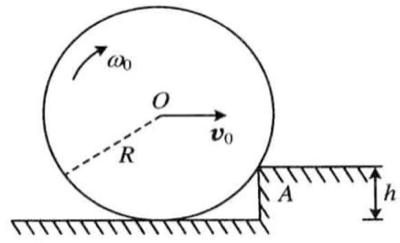
\includegraphics[width=0.3\linewidth,height=0.6\textheight,keepaspectratio]{figures/力图6-6-1.png}\\[2pt]
\textit{力图6-6-1}
\end{tabular}
\end{center}
\vfill
\newpage

\textbf{6-7} 如力图6-7-1，地球和月球的质量分别为 $M_{E}$ 和 $M_{m}$ ,两者中心的距离用 r 表示,月球可看作质点．设地球的自转轴和月球绕地球作圆周运动的转轴重合，都通过地球中心，地球和月球的角速度分别为 $\omega_{E}$ 和 $\omega_{m}$ ．由于潮汐运动，地球自转角速度会发生微小变化，从而地球和月球的间距以及地球和月球系统的总能量也将发生变化．

1. 试证明, 地球和月球间距的时间变化率 $\dot{r}$ 与地球自转角速度的时间变化率 $\omega_{E}$ 的关系为

$$
\dot {r} = - \frac {2 \sqrt {r} I _ {\mathrm{E}}}{M _ {\mathrm{m}} \sqrt {G M _ {\mathrm{E}}}} \dot {\omega} _ {\mathrm{E}}
$$

式中 $I_{E}$ 是地球对自转轴的转动惯量, G 是引力常量.

2. 试导出地球和月球系统机械能时间变化率的表达式。

3. 设现在的地球与月球间距为 $r(0)$ , 地球的自转角速度为 $\omega_{\mathrm{E}}(0)$ , 受扰动后相应的量变为 $r(t)$ 和 $\omega_{\mathrm{E}}(t)$ , 因扰动很小, 月球仍作圆周运动. 试证明

$$
\omega_ {\mathrm{E}} (t) = \omega_ {\mathrm{E}} (0) - \frac {M _ {\mathrm{m}} \sqrt {G M _ {\mathrm{E}}}}{I _ {\mathrm{E}}} [ \sqrt {r (t)} - \sqrt {r (0)} ]
$$

试计算地球和月球间距增加2\%时, 地球日将变成多少小时.



\begin{center}
\begin{tabular}{c}
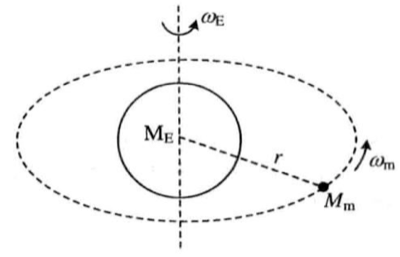
\includegraphics[width=0.3\linewidth,height=0.6\textheight,keepaspectratio]{figures/力图6-7-1.png}\\[2pt]
\textit{力图6-7-1}
\end{tabular}
\end{center}
\vfill
\newpage

\textbf{6-8} 某行星相对其质心轴的转动惯量为 $I$ ，自转角速度为 $\Omega$ 。质量为 $m$ 的卫星（可看作质点）绕该行星沿圆轨道运动，轨道半径为 $r$ ，角速度为 $\omega$ ，假定两种角速度的方向一致。

1. 一般情形下 $\Omega$ 与 $\omega$ 并不相等, 由于行星上的潮汐摩擦, 行星自转角速度将发生变化, 卫星的圆运动角速度也将相应地改变, 试求两种角速度的改变量之间的关系.

2. 潮汐摩擦将引起行星与卫星系统机械能的损耗, 试问在什么情形下系统机械能可达稳定值.
\vfill
\newpage

\textbf{6-9} 如力图6-9-1，一线轴质量为 $m$ ，绕质心轴的转动惯量为 $I$ ，大小半径分别为 $R$ 和 $r$ ，轴上绕线，以力 $F$ 拉线，拉力方向与水平面的夹角用 $\theta$ 表示。线轴放置在水平桌面上，与桌面之间的摩擦系数为 $\mu$ ，试讨论线轴的运动情况。



\begin{center}
\begin{tabular}{c}
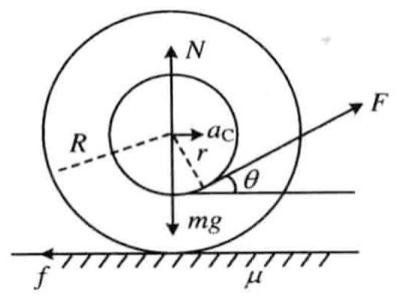
\includegraphics[width=0.3\linewidth,height=0.6\textheight,keepaspectratio]{figures/力图6-9-1.png}\\[2pt]
\textit{力图6-9-1}
\end{tabular}
\end{center}
\vfill
\newpage

\textbf{6-10} 如力图6-10-1，在 $\alpha = 30^{\circ}$ 的斜面上，质量 $m_{2} = 4\mathrm{kg}$ 的木块经轻绳与质量 $m_{1} = 8\mathrm{kg}$ 半径 $r = 5\mathrm{cm}$ 的实圆柱体的转轴相连。已知斜面的摩擦系数 $\mu = 0.2$ ，圆柱体轴承中的摩擦可以忽略。试求物体的加速度 $a$ ，并讨论加速度 $a$ 、张力 $T$ 、圆柱体所受摩擦力 $f_{1}$ 随斜面倾角 $\alpha$ 的变化。



\begin{center}
\begin{tabular}{c}
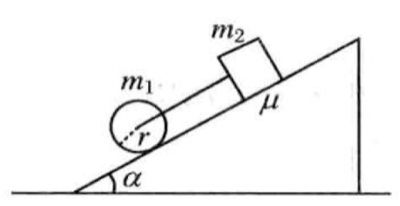
\includegraphics[width=0.3\linewidth,height=0.6\textheight,keepaspectratio]{figures/力图6-10-1.png}\\[2pt]
\textit{力图6-10-1}
\end{tabular}
\end{center}
\vfill
\newpage

\textbf{6-11} 如力图6-11-1，半径为 $R$ 的乒乓球，绕质心轴的转动惯量 $I = \frac{2}{3} mR^2, m$ 为乒乓球的质量，以一定的初始条件在粗糙的水平面上运动。开始时球的质心速度为 $v_{\mathrm{C0}}$ ，初角速度为 $\omega_0$ ，两者的方向如图所示。已知乒乓球与地面之间的摩擦系数为 $\mu$ 。试求乒乓球开始作纯滚运动所需的时间及纯滚时的质心速度。



\begin{center}
\begin{tabular}{c}
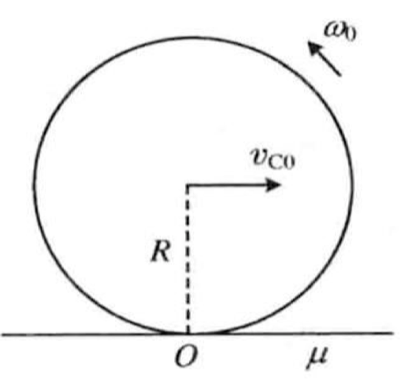
\includegraphics[width=0.3\linewidth,height=0.6\textheight,keepaspectratio]{figures/力图6-11-1.png}\\[2pt]
\textit{力图6-11-1}
\end{tabular}
\end{center}
\vfill
\newpage

\textbf{6-12} 如力图6-12-1，实心圆柱体从高度为 $h$ 的斜坡上从静止纯滚动地到达水平地面上, 继续纯滚动, 与光滑竖直墙作完全弹性碰撞后返回, 经足够长的水平距离后重新作纯滚动, 并纯滚动地爬上斜坡. 设地面与圆柱体之间的摩擦系数为 $\mu$ , 试求圆柱体爬坡所能达到的高度 $h'$ .



\begin{center}
\begin{tabular}{c}
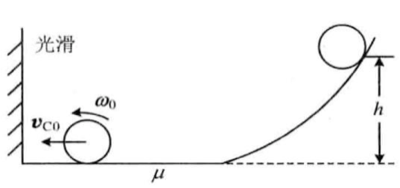
\includegraphics[width=0.3\linewidth,height=0.6\textheight,keepaspectratio]{figures/力图6-12-1.png}\\[2pt]
\textit{力图6-12-1}
\end{tabular}
\end{center}
\vfill
\newpage

\textbf{6-13} 如力图6-13-1，实心均匀小球自圆柱面的顶端从静止下滚.

1. 为了保证在 $\varphi \leqslant 45^{\circ}$ 的范围内小球作纯滚动, 试问摩擦系数 $\mu$ 至少应为多少.

2. 设 $\mu = 0.7$ , 试求纯滚结束时小球的质心速度 $v_{1}$.

3. 试求小球从圆柱面脱离时小球的位置 (用 $\varphi$ 角表示) 所满足的方程 (不必求解).



\begin{center}
\begin{tabular}{c}
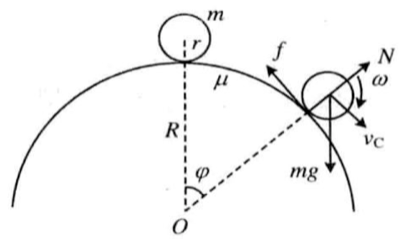
\includegraphics[width=0.3\linewidth,height=0.6\textheight,keepaspectratio]{figures/力图6-13-1.png}\\[2pt]
\textit{力图6-13-1}
\end{tabular}
\end{center}
\vfill
\newpage

\textbf{6-14} 在水平地面上有两个完全相同的均匀实心球，其一作纯滚动，质心速度为 $v$ ，另一静止不动。两球作完全弹性碰撞，因碰撞时间很短，碰撞过程中摩擦力的影响可以忽略不计。

试求: 1. 碰后两球达到纯滚时的质心速度. 2. 全部过程中损失的机械能的百分数.
\vfill
\newpage

\textbf{6-15} 如力图6-15-1，两个质量和半径均相同的实心圆柱轮，它们的质心轴互相平行，并用一轻杆相连，轴与轴承间的摩擦忽略不计。两轮先以共同的初速 $v_{0}$ 沿水平方向运动，两轮的初角速度为零。然后同时轻轻与地面相接触。设两轮与地面之间的摩擦系数分别为 $\mu_{1}$ 和 $\mu_{2}(\mu_{1}>\mu_{2})$ 。试求两轮均变为纯滚动所需的时间及纯滚后的平动速度。



\begin{center}
\begin{tabular}{c}
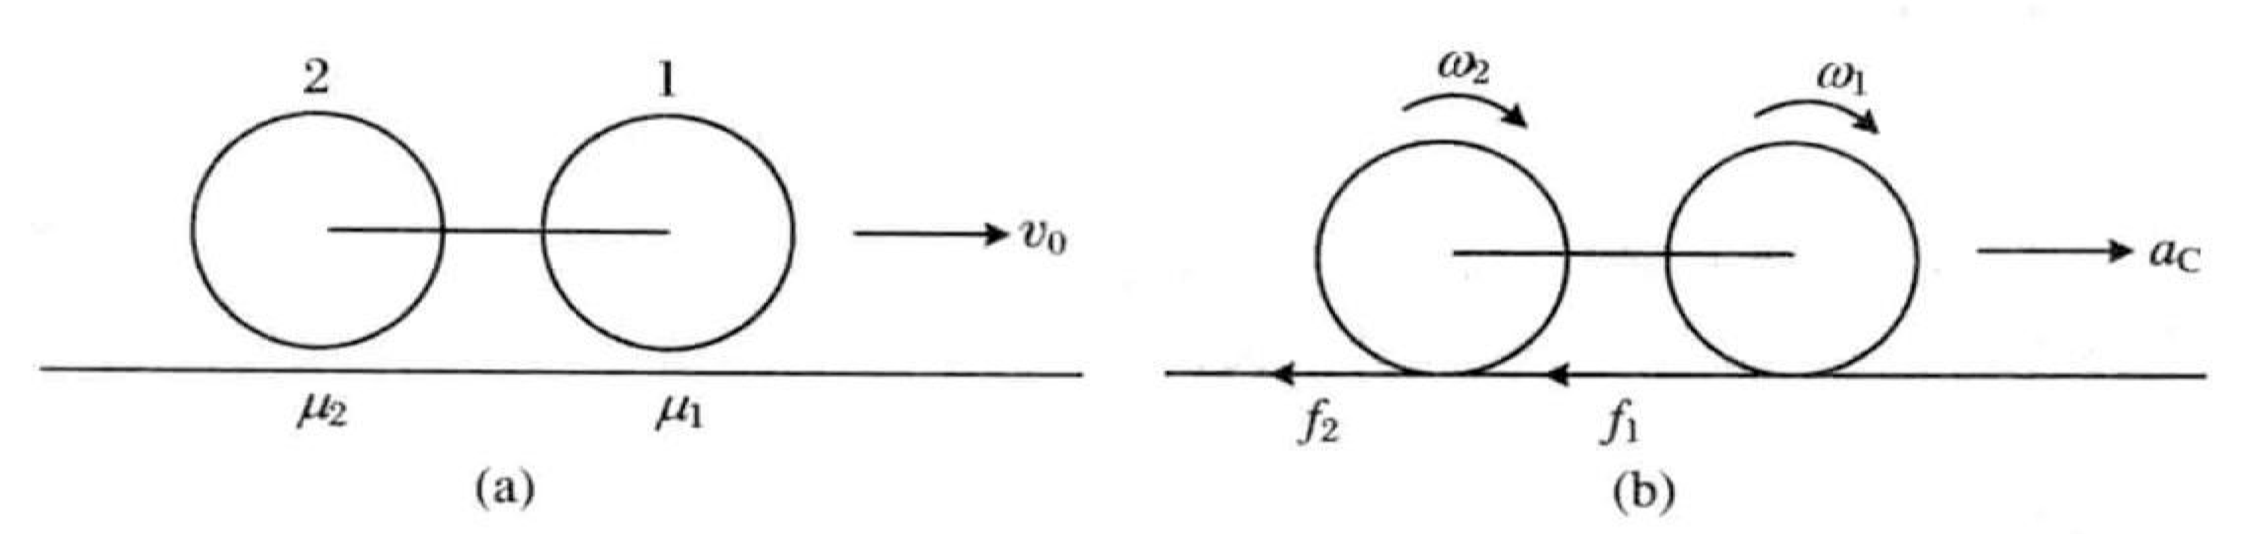
\includegraphics[width=0.3\linewidth,height=0.6\textheight,keepaspectratio]{figures/力图6-15-1.png}\\[2pt]
\textit{力图6-15-1}
\end{tabular}
\end{center}
\vfill
\newpage

\textbf{6-16} 如力图6-16-1，一半径为 $R$ 的实心均匀球，开始时质心静止，但绕通过质心的水平轴以角速度 $\omega_{0}$ 旋转，在重力作用下垂直下落到地面，球上最低点离地面的高度为 $h$。球与地面碰撞的恢复系数为 $e$，球与地面之间的摩擦系数为 $\mu$ ，忽略空气阻力及碰撞时产生的形变。

1. 试求碰地后球的质心速度和自转角速度。

2. 试求第一次落地点与第二次落地点之间的水平距离。

3. 试画出碰后球的质心速度与地面夹角 $\theta$ 的正切与初始角速度 $\omega_0$ 的关系曲线。



\begin{center}
\begin{tabular}{c}
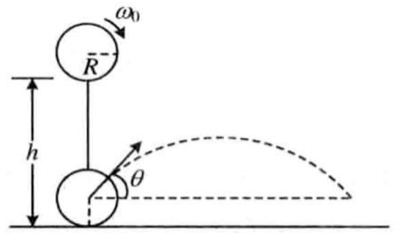
\includegraphics[width=0.3\linewidth,height=0.6\textheight,keepaspectratio]{figures/力图6-16-1.png}\\[2pt]
\textit{力图6-16-1}
\end{tabular}
\end{center}
\vfill
\newpage

\textbf{6-17} 如力图6-17-1，斜面体放置在光滑水平面上，斜面倾角为 $\theta$ ，一半径为 $R$ 的圆柱体在斜面上无滑动地下滚。设斜面体和圆柱体具有相同的质量 $m$ ，试求斜面体的加速度。



\begin{center}
\begin{tabular}{c}
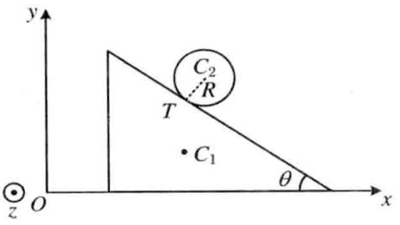
\includegraphics[width=0.3\linewidth,height=0.6\textheight,keepaspectratio]{figures/力图6-17-1.png}\\[2pt]
\textit{力图6-17-1}
\end{tabular}
\end{center}
\vfill
\newpage

\textbf{6-18} 如力图6-18-1，实心球在水平面内运动，质心的初始速度为 $\nu_{0}$ , 绕质心 $C$ 转动的初始角速度为 $\omega_{0}$ , 球与水平面之间的摩擦系数为 $\mu$ . 试分析球在水平面内的运动.



\begin{center}
\begin{tabular}{c}
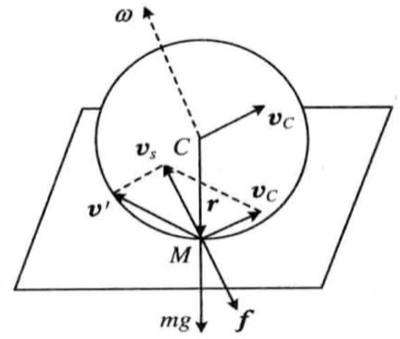
\includegraphics[width=0.3\linewidth,height=0.6\textheight,keepaspectratio]{figures/力图6-18-1.png}\\[2pt]
\textit{力图6-18-1}
\end{tabular}
\end{center}
\vfill
\newpage

\textbf{6-19} 如力图6-19-1，一个质量为 $m$ , 半径为 $R_A$ 的均匀圆盘 $A$ 在光滑水平面 $Oxy$ 内以速度 $V$ 沿 $x$ 方向平动, 圆盘中心至 $x$ 轴的垂直距离为 $b$ . 圆盘 $A$ 与另一静止的、其中心位于坐标原点 $O$ 的均匀圆盘 $B$ 相碰. 圆盘 $B$ 的质量与 $A$ 相同, 半径为 $R_B$ . 假定碰撞后两圆盘接触处的切向速度分量相等, 并假定碰撞前、后两盘沿连心线方向的相对速度大小不变. 试求:

1. 碰后两圆盘质心速度的 $x$ 分量和 $y$ 分量 $V_{Ax}^{\prime}, V_{Ay}^{\prime}, V_{Bx}^{\prime}, V_{By}^{\prime}$ .

2. 碰后两圆盘的动能 $E_A'$ 和 $E_B'$ .



\begin{center}
\begin{tabular}{c}
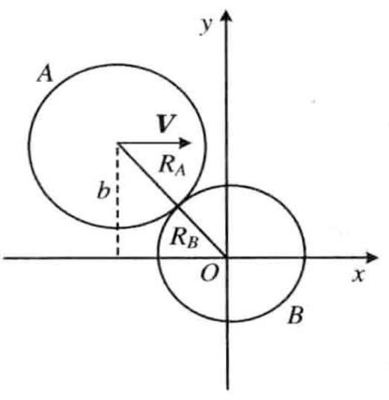
\includegraphics[width=0.3\linewidth,height=0.6\textheight,keepaspectratio]{figures/力图6-19-1.png}\\[2pt]
\textit{力图6-19-1}
\end{tabular}
\end{center}
\vfill
\newpage

\textbf{6-20} 如力图6-20-1，均匀细圆环半径为 $R$ ，质量为 $m$ ，平放在水平桌面上，与桌面之间的摩擦系数为 $\mu$ 。圆环质心 $O$ 沿 $x$ 轴以初速 $v_{\mathrm{C}0}$ 运动，同时圆环绕质心以初角速度 $\omega_0$ 顺时针转动， $v_{\mathrm{C}0}$ 与 $\omega_0$ 满足 $v_{\mathrm{C}0} = R\omega_0$ 。

试求: 1. 圆环所受摩擦力及摩擦力对质心的力矩. 2. 从开始到圆环停止运动所需时间.



\begin{center}
\begin{tabular}{c}
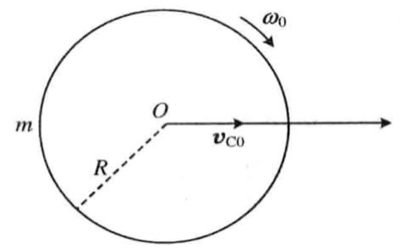
\includegraphics[width=0.3\linewidth,height=0.6\textheight,keepaspectratio]{figures/力图6-20-1.png}\\[2pt]
\textit{力图6-20-1}
\end{tabular}
\end{center}
\vfill
\newpage

\textbf{6-21} 长为 $l$ 的均匀细杆竖直地放置在光滑地面上，从静止倒下．试求落到地面时的质心速度.

\begin{center}
\begin{tabular}{c}
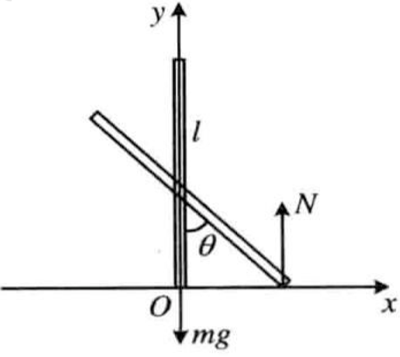
\includegraphics[width=0.3\linewidth,height=0.6\textheight,keepaspectratio]{figures/力图6-21-1.png}\\[2pt]
\textit{力图6-21-1}
\end{tabular}
\end{center}
\vfill
\newpage

\textbf{6-22} 如力图6-22-1，光滑水平地面上静止地放着质量为 $M$ 、长为 $l$ 的均匀细杆。质量为 $m$ 的质点以垂直于杆的水平初速 $\upsilon_0$ 与杆的一端作完全弹性碰撞.

试求: 1. 碰后系统质心的速度及绕质心的角速度. 2. 实际的转轴(即静止点)位于何处.



\begin{center}
\begin{tabular}{c}
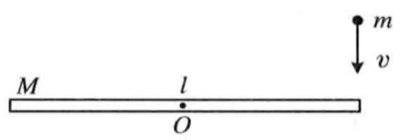
\includegraphics[width=0.3\linewidth,height=0.6\textheight,keepaspectratio]{figures/力图6-22-1.png}\\[2pt]
\textit{力图6-22-1}
\end{tabular}
\end{center}
\vfill
\newpage

\textbf{6-23} 如力图6-23-1，长为 $2l$ 的均匀细杆，下端支在地面上，上端靠在竖直墙上，从静止下滑，开始时杆与地面的夹角为 $\theta_0$ 。设杆与地和墙之间的摩擦可略。试问质心下降到初始高度的几分之几时，杆的上端与墙脱离。



\begin{center}
\begin{tabular}{c}
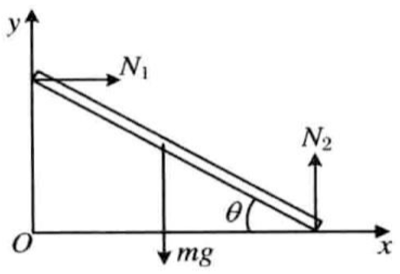
\includegraphics[width=0.3\linewidth,height=0.6\textheight,keepaspectratio]{figures/力图6-23-1.png}\\[2pt]
\textit{力图6-23-1}
\end{tabular}
\end{center}
\vfill
\newpage

\textbf{6-24} 如力图6-24-1，在光滑地面上静止地放置着两根质量均为 $m$ ，长度均为 $l$ 的均匀细杆.其中一杆由相等的两段构成，中间用光滑的铰链连接起来.在两杆的一端，各施以相同的垂直于杆的水平冲量 $J$ .试求两杆所获动能之比.



\begin{center}
\begin{tabular}{c}
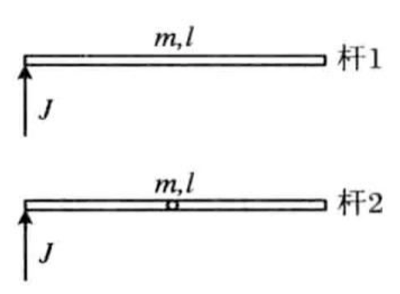
\includegraphics[width=0.3\linewidth,height=0.6\textheight,keepaspectratio]{figures/力图6-24-1.png}\\[2pt]
\textit{力图6-24-1}
\end{tabular}
\end{center}
\vfill
\newpage

\textbf{6-25} 如力图6-25-1，半径为 $R$ 的圆环绕铅垂的直径轴以角速度 $\omega$ 匀角速旋转。一细杆长 $L = \sqrt{2} R$ , 其两端约束在圆环上可作无摩擦滑动, 细杆的位置用 $OC$ 与铅垂轴的夹角 $\theta$ 表示, $C$ 为细杆的质心。试求细杆在圆环上的平衡位置, 并讨论平衡的稳定性。



\begin{center}
\begin{tabular}{c}
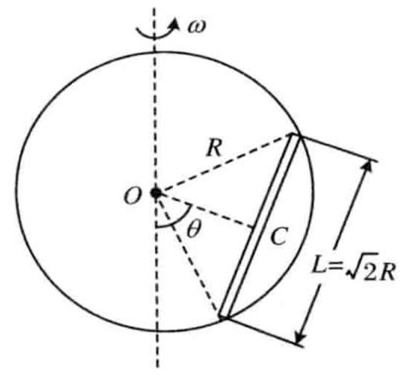
\includegraphics[width=0.3\linewidth,height=0.6\textheight,keepaspectratio]{figures/力图6-25-1.png}\\[2pt]
\textit{力图6-25-1}
\end{tabular}
\end{center}
\vfill
\newpage

\textbf{6-26} 如力图6-26-1， $Ox$ 和 $Oy$ 分别是支架的水平臂和铅垂臂， $Ox$ 臂绕铅垂臂作匀角速转动，角速度为 $\omega$ 。一均匀细杆的两端 $A$ 和 $B$ 被分别约束在两臂上运动，假定约束是理想的，细杆的质量为 $m$ ，长为 $2L$ ，细杆位置用图中 $\theta$ 角表示， $\theta$ 角是 $OC$ 与 $Oy$ 之间的夹角， $C$ 为细杆质心。以支架为参考系考察细杆的运动。

1. 试写出细杆的能量表达式。2. 试求细杆的平衡位置，并讨论平衡的稳定性。



\begin{center}
\begin{tabular}{c}
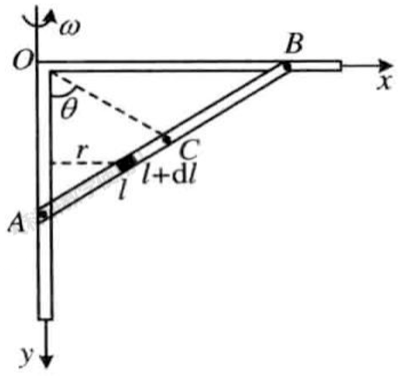
\includegraphics[width=0.3\linewidth,height=0.6\textheight,keepaspectratio]{figures/力图6-26-1.png}\\[2pt]
\textit{力图6-26-1}
\end{tabular}
\end{center}
\vfill
\newpage



\chapter{振动与波动}
\textbf{7-1} 如力图7-1-1，质量为 $m$ 、劲度系数为 $k$ 的弹簧振子放在光滑的水平面上，其平衡位置在 $O$ 点，其圆频率 $\omega = 0.5\pi \mathrm{rad}\cdot \mathrm{s}^{-1}$ 。另一质量亦为 $m$ 的质点放在光滑曲面的 $A$ 点， $AB$ 间高度差 $h = 0.20\mathrm{m}$ ，质点由 $A$ 点滑到 $B$ 点所需时间 $t_{AB} = 1.5\mathrm{s}, OB$ 之间的距离 $l = 6.0\mathrm{m}$ 。现将弹簧振子向左压缩到 $x_0 = 2.0\mathrm{m}$ 处自由释放，同时释放 $A$ 处的质点 $m$ ，两个质点相遇作完全非弹性碰撞后粘在一起，发生碰撞时弹簧作用力可略。若从碰撞开始计时，试求系统振动的数学表达式。（取 $g = 10\mathrm{m / s^2}$ ）。



\begin{center}
\begin{tabular}{c}
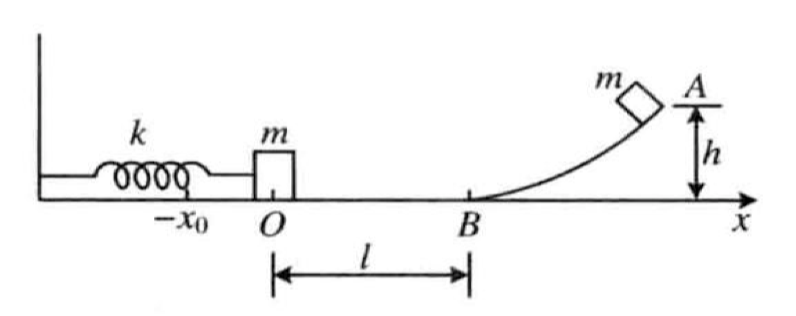
\includegraphics[width=0.3\linewidth,height=0.6\textheight,keepaspectratio]{figures/力图7-1-1.png}\\[2pt]
\textit{力图7-1-1}
\end{tabular}
\end{center}
\vfill
\newpage

\textbf{7-2} 如力图7-2-1,某液体的密度随深度线性地增加,液体表面的密度为 $\rho_{0}$ , 深度为 D 处的密度为 $2\rho_{0}$ , 一密度为 $2\rho_{0}$ 的小球在深度为 $\frac{D}{2}$ 处从静止释放. 忽略液体的阻力. 试求小球的振动表达式.



\begin{center}
\begin{tabular}{c}
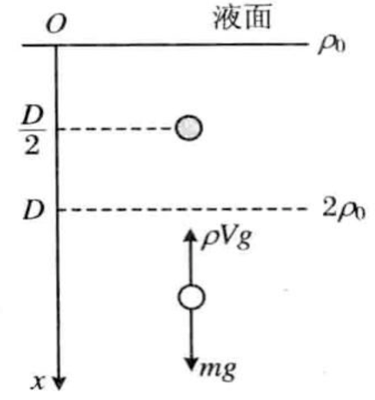
\includegraphics[width=0.3\linewidth,height=0.6\textheight,keepaspectratio]{figures/力图7-2-1.png}\\[2pt]
\textit{力图7-2-1}
\end{tabular}
\end{center}
\vfill
\newpage

\textbf{7-3} 如力图7-3-1,两个完全相同的圆柱状滚轮在水平面内平行放置,各绕自身的轴线按图示方向等角速转动,两轴线之间的距离为2l.在两滚轮上平放一块重量为G的均匀木板,木板与滚轮之间的摩擦系数为 $\mu$ .若木板重心偏离两轴中心位置一个微小的距离,试描述木板的运动.


\begin{center}
\begin{tabular}{c}
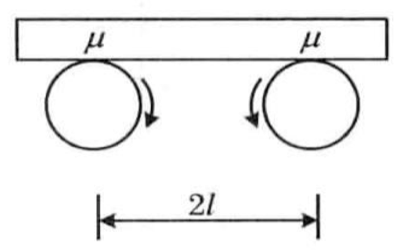
\includegraphics[width=0.3\linewidth,height=0.6\textheight,keepaspectratio]{figures/力图7-3-1.png}\\[2pt]
\textit{力图7-3-1}
\end{tabular}
\end{center}
\vfill
\newpage

\textbf{7-4} 牛顿曾证明：一个均匀球壳，对球壳内物质的万有引力为零，而对球壳外物质的万有引

力不为零, 并且其作用就相当于球壳的质量都集中到球心那样(参看力学第三章题11). 如力图7-4-1所示, 设想沿地球直径开凿一条贯通地球的隧道, 将一小球从洞口由静止释放, 试求小球到达隧道另一洞口所用的时间. 已知地球的半径为 $R$ , 质量为 $M$ , 设地球的质量均匀分布.

\begin{center}
\begin{tabular}{c}
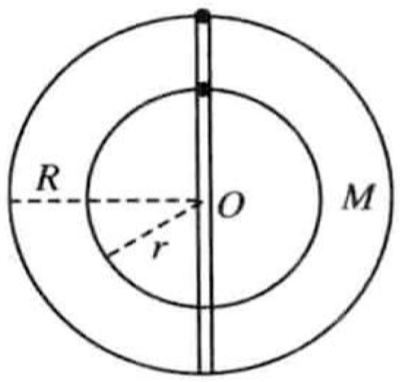
\includegraphics[width=0.3\linewidth,height=0.6\textheight,keepaspectratio]{figures/力图7-4-1.png}\\[2pt]
\textit{力图7-4-1}
\end{tabular}
\end{center}
\vfill
\newpage

\textbf{7-5} 如力图7-5-1，在倾角为 $\theta$ 的斜面上有一劲度系数为 $k$ 的弹簧，一端固定，另一端与质量为 $m$ 的实心圆柱体的轴连接，圆柱体在斜面上作纯滚动。忽略轴承的摩擦。试求振动周期。



\begin{center}
\begin{tabular}{c}
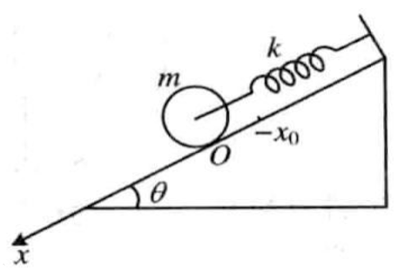
\includegraphics[width=0.3\linewidth,height=0.6\textheight,keepaspectratio]{figures/力图7-5-1.png}\\[2pt]
\textit{力图7-5-1}
\end{tabular}
\end{center}
\vfill
\newpage

\textbf{7-6} 如力图7-6-1，直角形均匀细杆的水平杆长为 $l$ 、质量为 $m$ ，竖直杆长为 $2l$ 、质量为 $2m$ ，细杆可绕拐角处的固定轴 $\mathcal{O}$ 无摩擦地转动．水平杆的一端与劲度系数为 $k$ 的弹簧相连，平衡时水平杆呈水平状态,竖直杆竖直下垂.试求微小摆动的周期.



\begin{center}
\begin{tabular}{c}
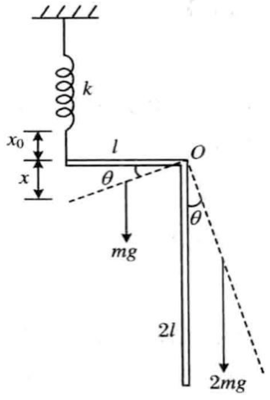
\includegraphics[width=0.3\linewidth,height=0.6\textheight,keepaspectratio]{figures/力图7-6-1.png}\\[2pt]
\textit{力图7-6-1}
\end{tabular}
\end{center}
\vfill
\newpage

\textbf{7-7} 如力图7-7-1, 弹簧振子中的小球质量为 $M$ , 弹簧的劲度系数为 $k$ , 弹簧的质量不可忽

略,设为 m, 假定弹簧的质量分布均匀, 忽略摩擦力. 试求振动周期.



\begin{center}
\begin{tabular}{c}
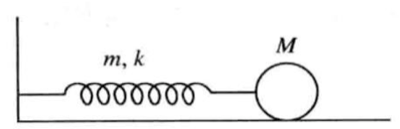
\includegraphics[width=0.3\linewidth,height=0.6\textheight,keepaspectratio]{figures/力图7-7-1.png}\\[2pt]
\textit{力图7-7-1}
\end{tabular}
\end{center}
\vfill
\newpage

\textbf{7-8} 如力图7-8-1，一不可伸长的细线穿过光滑桌面上的小孔，一端系质量为 $m$ 的小球，另一端系质

量为 M 的重物．小球在桌面上以角速度 $\omega_{0}$ 作匀速圆周运动，重物静止不动．若重物受到竖直向上或向下的扰动．试证明，重物将作上、下的简谐振动，并求振动圆频率．



\begin{center}
\begin{tabular}{c}
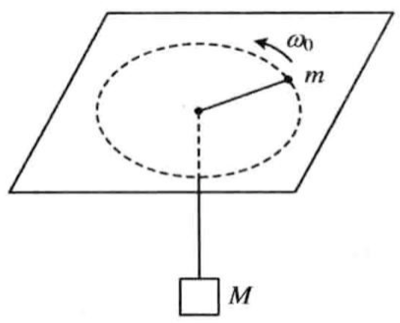
\includegraphics[width=0.3\linewidth,height=0.6\textheight,keepaspectratio]{figures/力图7-8-1.png}\\[2pt]
\textit{力图7-8-1}
\end{tabular}
\end{center}
\vfill
\newpage

\textbf{7-9} 如力图7-9-1，光滑的水平平板绕铅垂轴 $Oz$ 逆时针作匀角速转动，角速度为 $\omega$ 。在板面上，一质量可略、原长为 $l$ 、劲度系数为 $k$ 的弹簧一端固定在 $O$ 点，另一端系一质量为 $m$ 的小球。开始时小球位于 $(x_0,0)$ ，初速度为 $(v_0,0)$ 。试求小球相对平板的运动方程 $x = x(t), y = y(t)$ 。



\begin{center}
\begin{tabular}{c}
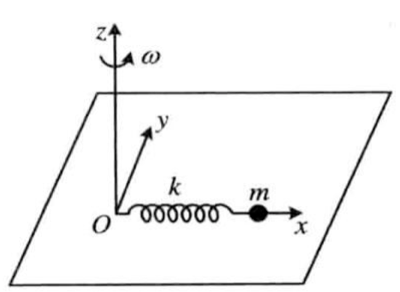
\includegraphics[width=0.3\linewidth,height=0.6\textheight,keepaspectratio]{figures/力图7-9-1.png}\\[2pt]
\textit{力图7-9-1}
\end{tabular}
\end{center}
\vfill
\newpage

\textbf{7-10} 在有些湖中，有时可观察到一种奇妙的湖震现象（水振荡）。通常是在一个浅的，长而比较窄的湖里可以看到。好像水的整体在运动，像你拿着一杯咖啡送到客人那里去时那样。不能把这种现象当作湖面上的水波。

我们用一只矩形容器作模型．容器的长度为 L，水高为 h．假定水面开始时与水平面成一小角度．水面开始振荡，振荡时水面仍保持平面，只是绕位于容器长度一半处的水平轴作振荡．

1. 试建立水运动的模型, 并求出振荡周期 $T$ 的表达式. 初始条件在力图7-10-1中给出. 假定 $\xi \ll h$ .

2. 下面两个表显示在两种不同长度的容器中, 不同深度的水

的振荡时间．以适当的方法检查你得出的公式,看它是否与实验数据很好吻合,并说明你对这种物理模型的适用性的意见．

\begin{center}
\begin{tabular}{cccc}
\hline
\multicolumn{2}{c}{力表7-10-1\quad $L=479$\,mm} & \multicolumn{2}{c}{力表7-10-2\quad $L=143$\,mm}\\
\hline
$h$/mm & $T$/s & $h$/mm & $T$/s\\
\hline
30 & 1.78 & 31 & 0.52\\
50 & 1.40 & 38 & 0.48\\
69 & 1.18 & 58 & 0.43\\
88 & 1.08 & 67 & 0.35\\
107 & 1.00 & 124 & 0.28\\
124 & 0.91 & & \\
142 & 0.82 & & \\
\hline
\end{tabular}
\end{center}

3. 力图 7-10-2 所示是在瑞典的 Vattern 湖上测量的结果, 两条曲线分别代表在湖的北端

Bastedalen 和南端 Jönköping 的测量．该湖长度为 123 km，平均深度为 50 m．在此情况下，时间标度应是什么？



\begin{center}
\begin{tabular}{c}
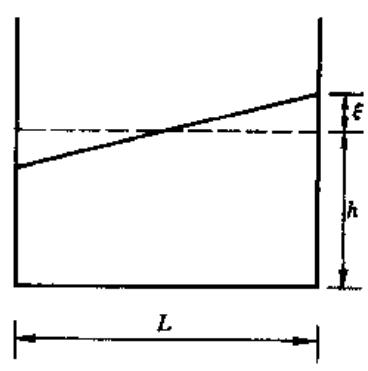
\includegraphics[width=0.3\linewidth,height=0.6\textheight,keepaspectratio]{figures/力图7-10-1.jpg}\\[2pt]
\textit{力图7-10-1}
\end{tabular}
\qquad
\begin{tabular}{c}
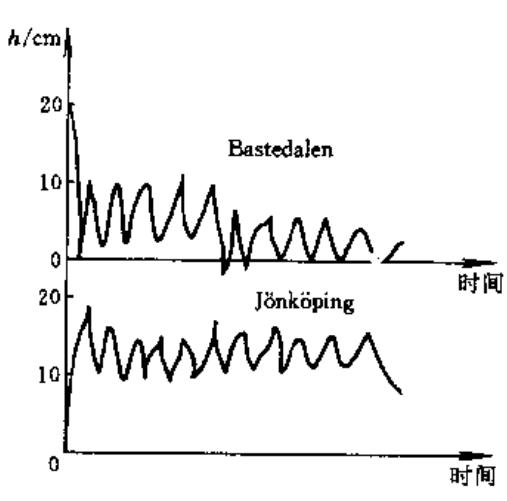
\includegraphics[width=0.3\linewidth,height=0.6\textheight,keepaspectratio]{figures/力图7-10-2.jpg}\\[2pt]
\textit{力图7-10-2}
\end{tabular}
\end{center}
\vfill
\newpage

\textbf{7-11} 如力图7-11-1，质量为 $m_{1}$ 的滑块可在光滑水平直导轨上滑动，滑块经长为 $l$ 质量可略的细杆

与质量为 $m_{2}$ 的重锤相连，细杆与重锤可绕滑块无摩擦地自由转动。设 $t = 0$ 时，细杆与导轨构成铅垂面，细杆与铅锤线夹角 $\theta_0$ ，从静止释放开始摆动。试求：1. 重锤 $m_{2}$ 的运动轨迹。2. 系统作小角摆动时，滑块位置随时间的变化。



\begin{center}
\begin{tabular}{c}
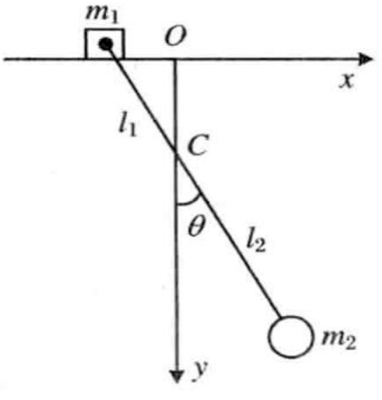
\includegraphics[width=0.3\linewidth,height=0.6\textheight,keepaspectratio]{figures/力图7-11-1.png}\\[2pt]
\textit{力图7-11-1}
\end{tabular}
\end{center}
\vfill
\newpage

\textbf{7-12} 如力图7-12-1,质量为 $m$ , 半径为 $r$ 的均匀实心小球在半径为 $R$ 的球形碗底作纯滚动. 试求微小振动的周期.



\begin{center}
\begin{tabular}{c}
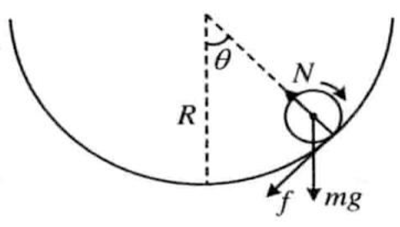
\includegraphics[width=0.3\linewidth,height=0.6\textheight,keepaspectratio]{figures/力图7-12-1.png}\\[2pt]
\textit{力图7-12-1}
\end{tabular}
\end{center}
\vfill
\newpage

\textbf{7-13} 如力图7-13-1, 质量为 $M$ 的物体放置在两个完全相同的质量均为 $m$ 的薄壁中空圆筒上. 物体两侧系着两个完全相同的劲度系数均为 $k$ 的弹簧, 两弹簧的另一端固定, 开始时两弹簧均为原长. 设物体在两薄圆筒上作纯滚动. 试求振动圆频率.



\begin{center}
\begin{tabular}{c}
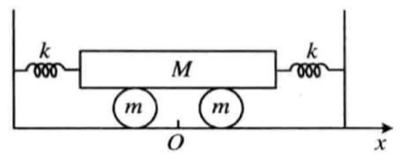
\includegraphics[width=0.3\linewidth,height=0.6\textheight,keepaspectratio]{figures/力图7-13-1.png}\\[2pt]
\textit{力图7-13-1}
\end{tabular}
\end{center}
\vfill
\newpage

\textbf{7-14} 如力图7-14-1，圆盘绕通过中心 $O$ 点的竖直轴在水平面内匀速转动，角速度为 $\omega$ ，质量为 $m$ 的小球被约束在圆盘上的光滑导轨 $AB$ 内运动。小球与一劲度系数为 $k$ 的弹簧相连 $(k > m\omega^2)$ ，弹簧另一端固定在圆盘 $A$ 点。弹簧为原长时，小球位于 $P$ 点， $OP = r_0$ ，且 $OP \perp AB$ ，将小球从 $P$ 点沿导轨拉开距离 $a$ 后从静止释放。在圆盘参考系中考察小球的运动。

1. 试求小球的平衡位置.2. 试证明小球作简谐振动,并求圆频率.3. 试求导轨施予小球的水平力随时间的变化规律.4. 试问当 $k < m\omega^2$ 时小球怎样运动.



\begin{center}
\begin{tabular}{c}
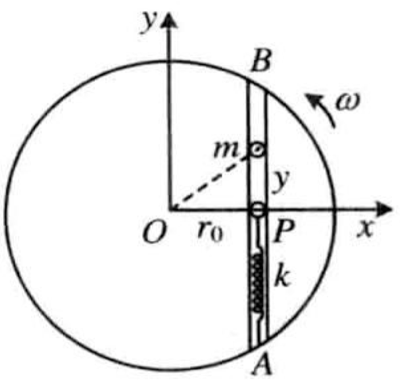
\includegraphics[width=0.3\linewidth,height=0.6\textheight,keepaspectratio]{figures/力图7-14-1.png}\\[2pt]
\textit{力图7-14-1}
\end{tabular}
\end{center}
\vfill
\newpage

\textbf{7-15} 如力图7-15-1，质量为 $m$ 的小球在光滑水平桌面上以角速度 $\omega$ 作匀速圆周运动。所需的向心力由与小球相连的弹簧提供，弹簧的劲度系数为 $k$ ，另一端固定。今沿径向轻击小球。试求小球径向振动的频率。



\begin{center}
\begin{tabular}{c}
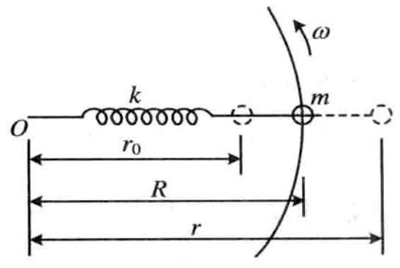
\includegraphics[width=0.3\linewidth,height=0.6\textheight,keepaspectratio]{figures/力图7-15-1.png}\\[2pt]
\textit{力图7-15-1}
\end{tabular}
\end{center}
\vfill
\newpage

\textbf{7-16} 计算单摆周期时，若摆幅 $\theta_0$ 较小，可采用一级近似 $\sin \theta \approx \theta$ ，算出的周期为 $T_{0} = 2\pi \sqrt{\frac{l}{g}}$ ，其中 $l$ 为摆长。若 $\theta_0$ 不算小，就应取二级近似。试导出单摆周期 $T$ 与摆幅 $\theta_0$ 的关系。
\vfill
\newpage

\textbf{7-17} 对于谐振子, 若广义动量为 $p$ , 广义坐标为 $q$ , 则有 $\oint p \mathrm{d} q = \frac{E}{\nu}$ , 其中 $E$ 为谐振子的能量, $\nu$ 为振动频率. 积分在振动的一个周期内进行. 试就弹簧振子和单摆的情况证明此式.
\vfill
\newpage

\textbf{7-18} 如力图7-18-1, $T$ 形导轨固定在铅垂面内, 质量为 $m$ 、全长为 $l$ 的刚性均匀细杆两端约束在 $T$ 形导轨中, 可沿导轨作无摩擦的滑动. 1. 试求细杆作小振幅摆动时的振动周期. 2. 当细杆摆至右方适当角度刚好达到静止时 (如力图7-18-1中虚线所示), 一质量也为 $m$ 的小球以速度 $v_{0}$ 沿水平方向经导轨与细杆上端相碰. 设碰撞无机械能损失, 碰后小球速度变为零, 细杆则回摆到左方与水平导轨平行时刚好静止. 试问 $v_{0}$ 应为多大?



\begin{center}
\begin{tabular}{c}
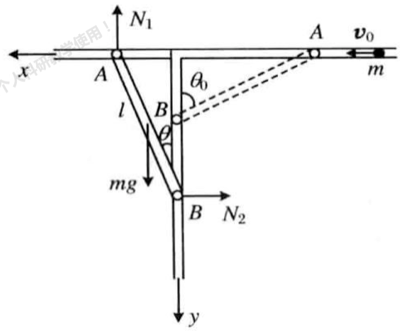
\includegraphics[width=0.3\linewidth,height=0.6\textheight,keepaspectratio]{figures/力图7-18-1.png}\\[2pt]
\textit{力图7-18-1}
\end{tabular}
\end{center}
\vfill
\newpage

\textbf{7-19} 如力图7-19-1，在光滑水平面上，质量为 $m_{1}$ 和 $m_{2}$ 的两物体用劲度系数为 $k$ 的弹簧相连。当弹簧为原长时， $m_{1}$ 与 $m_{2}$ 相距 $l_{0}$ ，把弹簧压缩距离 $a$ 后从静止释放。试求 $m_{1}$ 和 $m_{2}$ 的振动表达式。



\begin{center}
\begin{tabular}{c}
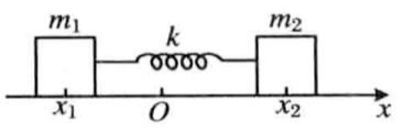
\includegraphics[width=0.3\linewidth,height=0.6\textheight,keepaspectratio]{figures/力图7-19-1.png}\\[2pt]
\textit{力图7-19-1}
\end{tabular}
\end{center}
\vfill
\newpage

\textbf{7-20} 如力图7-20-1，单摆的原长为 $l_{0}$ ，在摆动过程中缓慢上拉，悬点位置不变而摆长逐渐缩短。试求

当摆长缩短为原长之半，即 $l = \frac{l_0}{2}$ 时的振幅与原振幅之比。



\begin{center}
\begin{tabular}{c}
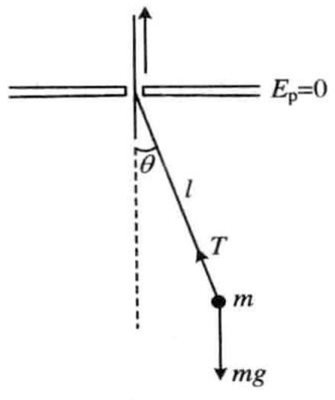
\includegraphics[width=0.3\linewidth,height=0.6\textheight,keepaspectratio]{figures/力图7-20-1.png}\\[2pt]
\textit{力图7-20-1}
\end{tabular}
\end{center}
\vfill
\newpage

\textbf{7-21} 如力图7-21-1，质量为 $M$ 、长为 $L$ 的均匀刚性细杆的一端悬挂，可在铅垂面内绕悬点无摩擦地

摆动．质量为 $m=\frac{M}{3}$ 的小虫相对杆以速度 $v_{s}$ 缓慢地沿杆向下爬行．开始时，杆静止并与竖直线夹 $\theta_{0}$ 角（设 $\theta_{0}$ 很小）；小虫位于杆上端的悬点．放开后，杆开始摆动，小虫开始爬行．

试求:1. 小虫沿杆爬行 l 距离时,杆摆动的圆频率.2. 小虫爬到杆下端时,杆摆动的幅度.



\begin{center}
\begin{tabular}{c}
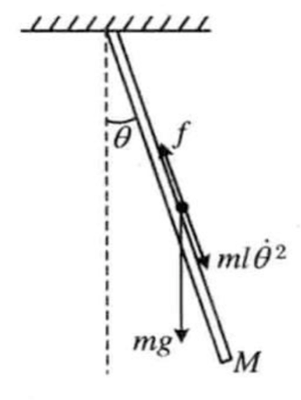
\includegraphics[width=0.3\linewidth,height=0.6\textheight,keepaspectratio]{figures/力图7-21-1.png}\\[2pt]
\textit{力图7-21-1}
\end{tabular}
\end{center}
\vfill
\newpage

\textbf{7-22} 如力图7-22-1，圆盘在水平面内以匀角速 $\Omega$ 绕竖直轴 $OO'$ 旋转，盘上固连着两根同样高度的竖直支架。质量为 $m$ 的小球与质量可忽略不计的 $T$ 字形细杆相连，水平杆由支架支承，与小球相连的杆长为 $l$ ，悬点 $O'$ 在转轴上，整个系统可在支架上无摩擦地摆动。

试求:1. 小球的平衡位置.2. 小球作小幅摆动时的圆频率.



\begin{center}
\begin{tabular}{c}
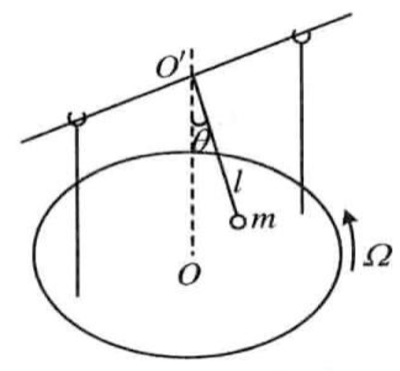
\includegraphics[width=0.3\linewidth,height=0.6\textheight,keepaspectratio]{figures/力图7-22-1.png}\\[2pt]
\textit{力图7-22-1}
\end{tabular}
\end{center}
\vfill
\newpage

\textbf{7-23} 如力图7-23-1，在光滑水平面上有三质点 $A, B, C$ ，质量分别为 $m_1, m_2$ 和 $m_3$ ，三质点位于同一直线上，开始时 $B$ 和 $C$ 静止，用劲度系数为 $k$ 的弹簧（质量忽略）相连。质点 $A$ 以初速 $v_0$ 沿连线方向与 $B$ 作完全弹性碰撞。



1. 以 $A$ 和 $B$ 的碰撞点为坐标原点, 连线为 $x$ 轴, 试求碰后质点 $B$ 的运动规律. 2. 设 $m_2 = m_3 = m$ , 为使质点 $A$ 和 $B$ 在碰后重新相遇, 但不相碰 (即相遇时速度相同), 试问比值 $\frac{m_1}{m}$ 应为多少?



\begin{center}
\begin{tabular}{c}
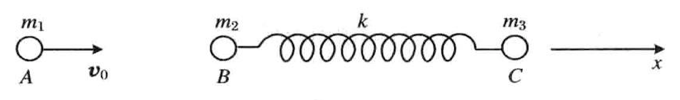
\includegraphics[width=0.3\linewidth,height=0.6\textheight,keepaspectratio]{figures/力图7-23-1.png}\\[2pt]
\textit{力图7-23-1}
\end{tabular}
\end{center}
\vfill
\newpage

\textbf{7-24} 如力图7-24-1，质量为 $M$ 的小球两侧分别用劲度系数均为 $k$ 的弹簧与两个质量均为 $m$ 的小球连成一直线，水平放置，忽略一切阻力和摩擦力。试求特征频率和振动模式。

\begin{center}
\begin{tabular}{c}
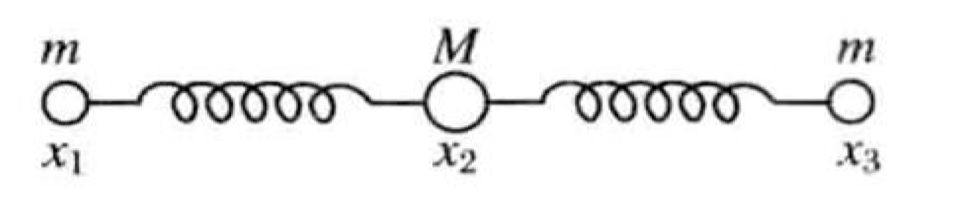
\includegraphics[width=0.3\linewidth,height=0.6\textheight,keepaspectratio]{figures/力图7-24-1.png}\\[2pt]
\textit{力图7-24-1}
\end{tabular}
\end{center}
\vfill
\newpage
\textbf{7-25} 如力图7-25-1，质量为 $m$ 、长为 $l$ 的均匀长方形木板由劲度系数分别为 $k_{1}$ 和 $k_{2}$ 的两竖直弹簧在两端支撑，平衡时木板位于水平面。试求木板作小幅振动时的特征频率。



\begin{center}
\begin{tabular}{c}
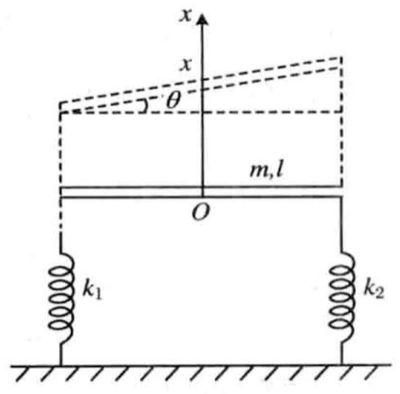
\includegraphics[width=0.3\linewidth,height=0.6\textheight,keepaspectratio]{figures/力图7-25-1.png}\\[2pt]
\textit{力图7-25-1}
\end{tabular}
\end{center}
\vfill
\newpage

\textbf{7-26} 如力图7-26-1,两个完全相同的单摆并排悬挂,摆球质量均为 $m$ ,摆长均为 $l$ ,两摆球用劲度系数为 $k$ 的轻质弹簧连接,弹簧原长等于两悬点之间的距离.忽略空气阻力.上述振

动系统称为耦合摆．在小角摆动的条件下，1. 试求耦合摆的特征频率，并写出两摆球运动方程的一般表达式．2. 试讨论耦合摆在不同初始条件下的几种典型运动情况．



\begin{center}
\begin{tabular}{c}
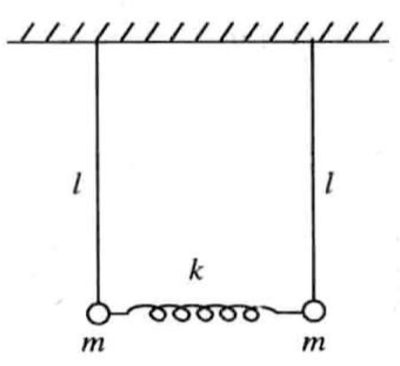
\includegraphics[width=0.3\linewidth,height=0.6\textheight,keepaspectratio]{figures/力图7-26-1.png}\\[2pt]
\textit{力图7-26-1}
\end{tabular}
\end{center}
\vfill
\newpage

\textbf{7-27} 如力图7-27-1，6个质量均为 $m$ 的小球串在光滑圆环上，彼此间用劲度系数均为 $k$ 的6个弹簧相连，整个系统在水平面内。当各小球处在平衡位置时，弹簧均为原长。试求特征频率。



\begin{center}
\begin{tabular}{c}
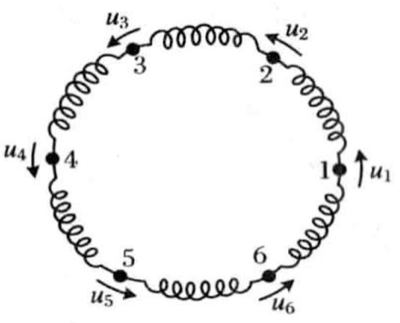
\includegraphics[width=0.3\linewidth,height=0.6\textheight,keepaspectratio]{figures/力图7-27-1.png}\\[2pt]
\textit{力图7-27-1}
\end{tabular}
\end{center}
\vfill
\newpage

\textbf{7-28} 三个质量各为 $m$ 的质点由未伸长的无质量弹簧连接在一起达到平衡。每个弹簧的劲度系数为 $k$ ，它们被限制在圆周上运动，如力图7-28-1所示。

1. 若每一质点 $m$ 分别有偏离平衡位置的小位移 $u_{1}, u_{2}$ 和 $u_{3}$ , 试写出每一质点的运动方程

2. 试验证此系统有下列简谐式解
$$
u _ {n} = a _ {n} \cos \omega t
$$
其加速度为 $-\omega^2 u_n$ ，此处 $a_n (n = 1,2,3)$ 是恒振幅，角频率 $\omega$ 有下列三个可能的取值，即
$$
\sqrt {3} \omega_ {0}, \sqrt {3} \omega_ {0}, 0
$$
其中 $\omega_{0}^{2}=\frac{k}{m}$ .

3. 将这由弹簧与质点交替连接的系统扩充到 N 个质点，每一质点 m 由弹簧与相邻质点连接。起初弹簧未伸长，处于平衡，当质点偏离平衡时，用第 n 个质点的位移和相邻质点的位移表示出第 n 个质点 $(n=1,2,\cdots,N)$ 的运动方程。试验证
$$
u _ {n} (t) = a _ {s} \sin \left(\frac {2 n s \pi}{N} + \varphi\right) \cos \omega_ {s} t
$$
是振荡解，式中 $s=1,2,\cdots,N,n=1,2,\cdots,N,\varphi$ 为一任意相位，角频率 $\omega_{s}$ 由下式给出
$$
\omega_ {s} = 2 \omega_ {0} \sin \left(\frac {s \pi}{N}\right)
$$
而 $a_{s}(s=1,2,\cdots,N)$ 是与 n 无关的恒振幅。

试叙述对于一个含有无穷多个质点的链条,频率的可能范围.

4. 试确定 $\frac{u_n}{u_{n+1}}$ 的比值。

当 $N$ 很大时, 对于下列 $(a), (b)$ 两种情况, 试画出说明时刻 $t$ 质点的位移与该质点在链上编号之间关系的草图.

(a)低频解.

$(b)\omega_{s}=\omega_{\max}$ ，其中 $\omega_{\max}$ 是最大的频率解。

5. 若质点之一用质量 $m^{\prime} \ll m$ 的质点代替, 试估计角频率分布将发生怎样的主要变化.

试在上面结果的基础上定性地描述,由质量为 m 和 $m'$ 交替联接的双原子链会有怎样形式的频谱.

提示：
$$
\begin{array}{r l} \sin (A + B) & = \sin A \cos B + \cos A \sin B \\ \sin A + \sin B & = 2 \sin \frac {A + B}{2} \cos \frac {A - B}{2} \\ 2 \sin^ {2} A & = 1 - \cos 2 A \end{array}
$$



\begin{center}
\begin{tabular}{c}
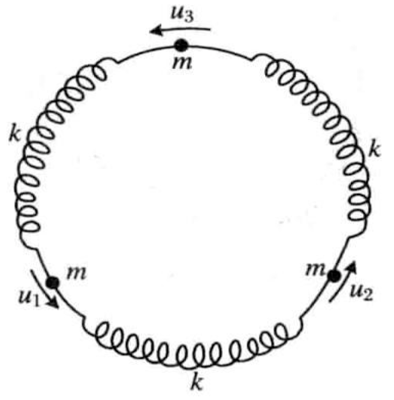
\includegraphics[width=0.16\linewidth,height=0.30\textheight,keepaspectratio]{figures/力图7-28-1.png}\\[2pt]
\textit{力图7-28-1}
\end{tabular}
\end{center}
\vfill
\newpage

\textbf{7-29} 如力图7-29-1，细杆长 $l$ ，上端 $O$ 悬挂，下端与质量为 $m$ 的摆球相连，摆球可绕 $O$ 轴无摩擦地摆动。今在细杆的 $A$ 点经连杆接一阻尼器，阻尼力 $f$ 沿水平方向，其大小

与阻尼板的速度 $v$ 成正比，即 $f = \gamma v, \gamma$ 为阻力系数。设 $OA = a$ ，细杆、连杆、阻尼板等的质量均远小于 $m$ ，可忽略不计，阻尼较弱。试求小幅阻尼振动的对数减缩，以及一周期内损失能量的百分比。



\begin{center}
\begin{tabular}{c}
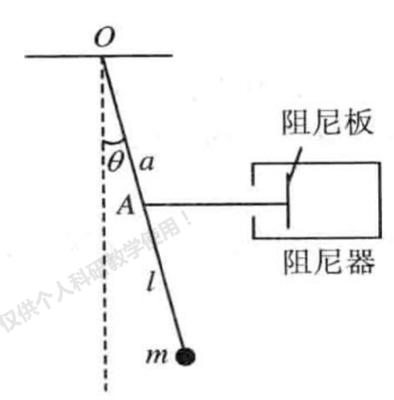
\includegraphics[width=0.3\linewidth,height=0.6\textheight,keepaspectratio]{figures/力图7-29-1.png}\\[2pt]
\textit{力图7-29-1}
\end{tabular}
\end{center}
\vfill
\newpage

\textbf{7-30} 质量为 $m$ 的质点在弹性力和阻尼力的作用下沿 $x$ 轴运动。取平衡位置为坐标原点，弹性力为 $-kx$ ，阻尼力为 $-\gamma x$ 。试问，是否在临界阻尼情况下，质点回到平衡位置一定最快？
\vfill
\newpage

\textbf{7-31} 如力图7-31-1，充满液体的容器在竖直方向上下振动，质量为 $m$ 的重物由劲度系数为 $k$ 的弹簧悬挂，浸没在液体之中。设悬点随容器振动的规律为 $x_{H} = A\cos \omega t$ ，设液体的阻尼系数为 $\gamma$ （弱阻尼），并假定液体的浮力恒定。

1. 若 $\omega = \omega_0$ ，试求稳定后重物的振动表达式，其中 $\omega_0 = \sqrt{\frac{k}{m}}$ 为弹簧振子的固有圆频率。

2. 若 $\omega \gg \omega_0$ ，试求稳定后重物的振动表达式。

3. 若 $\omega \gg \omega_{0}$ ，且当容器达到最高点时突然停止不动，试求此后重物的振动表达式。

4. 试画出容器突然停止以前和以后的振动曲线。



\begin{center}
\begin{tabular}{c}
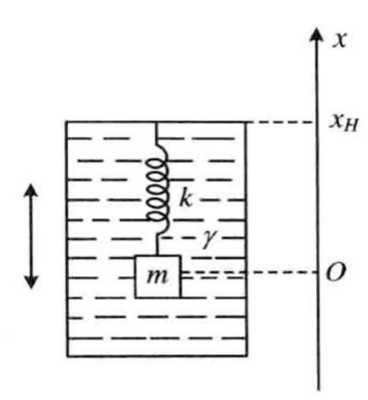
\includegraphics[width=0.3\linewidth,height=0.6\textheight,keepaspectratio]{figures/力图7-31-1.png}\\[2pt]
\textit{力图7-31-1}
\end{tabular}
\end{center}
\vfill
\newpage

\textbf{7-32} 如力图7-32-1，质量均为 $m$ 的三个滑块放置在光滑水平桌面上，彼此以原长为 $x_0$ 、劲度系数为

k 的二个相同弹簧连接起来。开始时三滑块静止，滑块 A 位于原点 O，两弹簧均为原长。对滑块 A 施以周期性外力 F，已知 $F = F_{0} \cos \omega t$ ，在水平方向并沿三滑块连线。试求振动系统的特征频率，并写出滑块 C 的运动方程。



\begin{center}
\begin{tabular}{c}
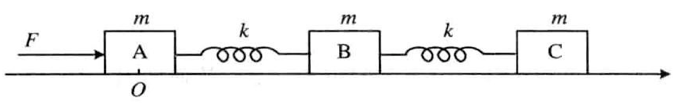
\includegraphics[width=0.3\linewidth,height=0.6\textheight,keepaspectratio]{figures/力图7-32-1.png}\\[2pt]
\textit{力图7-32-1}
\end{tabular}
\end{center}
\vfill
\newpage

\textbf{7-33} 本世纪初曾提出一种地球模型，认为它是一个半径为 $R$ 的球体，从地球表面向内到半

径 $R_{C}$ 处为均匀各向同性的固态地幔， $R_{C}$ 以内的地芯为液态，如力图 7-33-1 所示。

在地幔内,地震纵波 p 和横波 s 的速度分别为常量 $v_{p}$ 和 $v_{s}$ ; 在地芯内,纵波的速度为常量 $v_{Cp}$ , 且 $v_{Cp} < v_{p}$ , 而横波不传播.

在地球表面 E 处发生了一次地震, 产生的地震波在地球内传播, 且被地球表面 X 处设置有地震仪的观察者观察到 .E 点和 X 点的角间隔 $2\theta = \angle EOX$ , 其中 O 为地球中心.

1. 试证明, 对于 $\theta \leqslant \arccos \frac{R_C}{R}$ 的那些 $X$ 点, 从 $E$ 点发出的地震波沿直线穿过地幔传播到 $X$ 点的时间为 $t = \frac{2R\sin\theta}{v}$ , 对于 $p$ 波, $v = v_p$ , 对于 $s$ 波 $v = v_s$ .

2. 对于 $\theta > \arccos \frac{R_C}{R}$ 的那些 $X$ 点，地震 $p$ 波在地幔和地芯的界面上经过两次折射后到达 $X$ 点。画出这种地震 $p$ 波的传播路径，并求出对于 $p$ 波， $\theta$ 和 $i$ 之间的关系式，这里 $i$ 是 $p$ 波在地幔和地芯界面上的入射角。

3. 利用下列数据和第2问中所得结果，画出 $\theta \sim i$ 图形. $R = 6370\mathrm{km}, R_C = 3470\mathrm{km}, v_p = 10.85\mathrm{km/s}, v_s = 6.31\mathrm{km/s}, v_{Cp} = 9.02\mathrm{km/s}$ . 试评论，对于地球表面不同地点的观察者，从上述 $\theta \sim i$ 图形可得出什么物理结论.

4. 在一次地震后, 某观察者测出 $s$ 波相对 $p$ 波的时间延迟为 2 分 11 秒, 试用第 3 问中给出的数据确定地震地点与观察者之间的角间隔.

5. 在上述测量中, 观察者注意到某次 $p$ 波和 $s$ 波到达后, 地震仪上还有两个相间 6 分 37 秒的记录. 试解释这一结果, 并验证这与第 4 问所得的角间隔确实相符.

\begin{center}
\begin{tabular}{c}
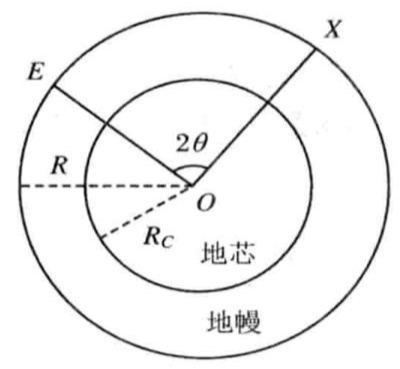
\includegraphics[width=0.3\linewidth,height=0.6\textheight,keepaspectratio]{figures/力图7-33-1.png}\\[2pt]
\textit{力图7-33-1}
\end{tabular}
\end{center}
\vfill
\newpage

\textbf{7-34} 到晚上,地面辐射降温使空气层产生温度梯度,温度随高度递增,这导致声速 $v$ 随高度 $y$ 变化.假定变化规律为

$$
v = v _ {0} (1 + a ^ {2} y ^ {2})
$$

式中 $v_{0}$ 是地面 $(y = 0)$ 处的声速， $\alpha$ 为比例系数。今远方地面上某声源发出一束声波，发射方向与竖直方向成 $\theta_{0}$ 角。假定在声波传播范围内 $\alpha y \ll 1$ 。试导出该束声波在空间传播所循的轨迹，并求地面上听得最清晰的地点与声源的距离。

\begin{center}
\begin{tabular}{c}
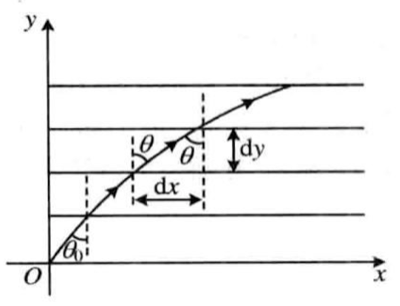
\includegraphics[width=0.3\linewidth,height=0.6\textheight,keepaspectratio]{figures/力图7-34-1.png}\\[2pt]
\textit{力图7-34-1}
\end{tabular}
\end{center}
\vfill
\newpage

\textbf{7-35} 在海洋中，声波的速度随深度、温度和含盐量变化。已知声速随深度变化的规律如力图7-35-1所示。最小声速 $v_{0}$ 出现在海洋表面和海底之间，以最小声速处作为坐标原点， $z_{s}$ 和 $z_{b}$ 分别表示海洋表面和海底的坐标，则声速v与z的关系为

$$
v = \left\{ \begin{array}{l l} v _ {0} + b z & (z > 0) \\ v _ {0} & (z = 0) \\ v _ {0} - b z & (z <   0) \end{array} \right.
$$

其中 $b$ 为正的常量.

如力图7-35-2，今在 $x = 0, z = 0$ 处放置一声源 $S$ 。在 $zx$ 平面内，从 $S$ 发出的声波的传播方向用初始发射角 $\theta_0$ 表示。声速的不均匀将导致波射线的弯曲。

1. 试证明在 $zx$ 平面内声波的初始轨迹是半径为 $R$ 的圆弧，且

$$
R = \frac {v _ {0}}{b \sin \theta_ {0}} \quad \left(0 \leqslant \theta_ {0} <   \frac {\pi}{2}\right)
$$

2. 在不被海洋表面反射的声波中, 最小的 $\theta_{0}$ 是什么?

3. 设在 Ox 轴上 x = X 处设置接收器 H，试导出能直接到达接收器的各声波所对应的 $\theta_{0}$ 的公式。（排除经海洋表面和海底而到达接收器的情形。）

4. 已知 $X = 10000 \mathrm{~m}, v_0 = 1500 \mathrm{~m/s}, b = 0.020 \mathrm{~s}^{-1}$ . 试用这些数据计算可使声波直接从 $S$ 传到 $H$ (不经反射) 的 4 个 $\theta_0$ 的值 (从最小的 $\theta_0$ 开始).

5. 当 $\theta_0$ 取第3问中得出的最小值时, 试导出声波从 $S$ 传播到 $H$ 所需时间的表达式, 并用第4问所给的数据算出这个传播时间. 再计算当 $\theta_0 = \frac{\pi}{2}$ 时, 即声波沿 $x$ 传播到 $H$ 所需的时间. 比较上述两个时间的大小.



\begin{center}
\begin{tabular}{c}
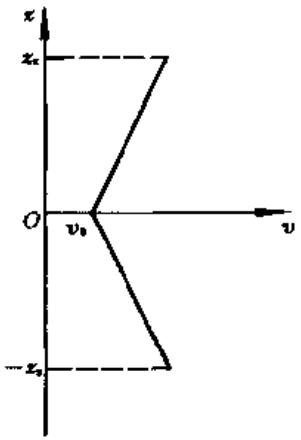
\includegraphics[width=0.21\linewidth,height=0.45\textheight,keepaspectratio]{figures/力图7-35-1.jpg}\\[2pt]
\textit{力图7-35-1}
\end{tabular}
\qquad
\begin{tabular}{c}
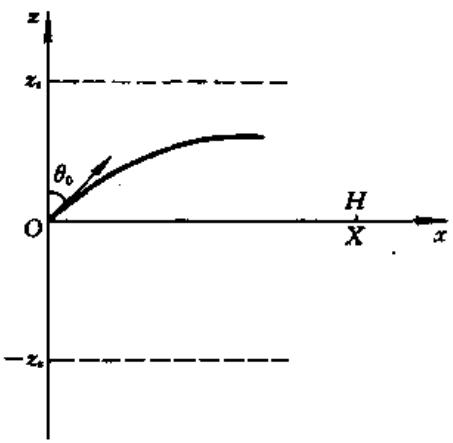
\includegraphics[width=0.21\linewidth,height=0.45\textheight,keepaspectratio]{figures/力图7-35-2.jpg}\\[2pt]
\textit{力图7-35-2}
\end{tabular}
\end{center}
\vfill
\newpage

\textbf{7-36} 如力图7-36-1,质量为 $m$ 、劲度系数为 $\pmb{k}$ 的弹簧原长为 $L$ ,一端固定,另一端与一质量为 $M$ 的物体相连,整个系统水平放置,物体 $M$ 可在光滑水平面上滑动.1.试导出纵向弹性波的波动方程并求波速.2.假定 $L$ 远小于弹性波的波长, $M$ 的振幅为 $A_0$ ,试求弹簧上各点的振幅分布.3.在 $m \ll M$ 的条件下,试分别求零级近似和一级近似的频率.



\begin{center}
\begin{tabular}{c}
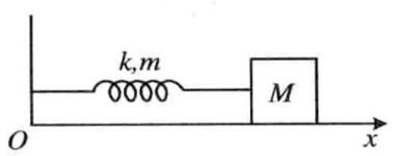
\includegraphics[width=0.3\linewidth,height=0.6\textheight,keepaspectratio]{figures/力图7-36-1.png}\\[2pt]
\textit{力图7-36-1}
\end{tabular}
\end{center}
\vfill
\newpage

\textbf{7-37} 无穷长弦线，拉紧，质量线密度为 $\rho = 0.01\mathrm{kg / m}$ 。今在线一端施以横向简谐力，峰值为 $F_{\max} = 0.3\mathrm{N}$ ，使弦线中产生简谐振动，波速为 $v = \frac{30}{\pi}\mathrm{m / s}$ 。试求单位时间内通过弦线某一截面传输的平均能量 $S$ 。

\begin{center}
\begin{tabular}{c}
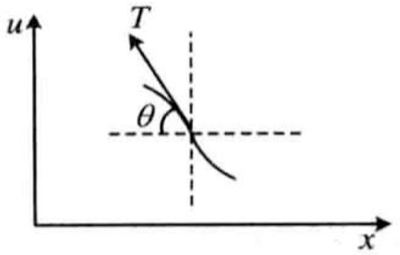
\includegraphics[width=0.3\linewidth,height=0.6\textheight,keepaspectratio]{figures/力图7-37-1.png}\\[2pt]
\textit{力图7-37-1}
\end{tabular}
\end{center}
\vfill
\newpage

\textbf{7-38} 拉紧的弦线，张力为 $T$ ，质量线密度为 $\rho$ ，质量为 $m$ 的质点附在弦上某点．圆频率为 $\omega$ 的波沿弦线传播．试求波在质点 $m$ 反射时的能量反射系数．

\begin{center}
\begin{tabular}{c}
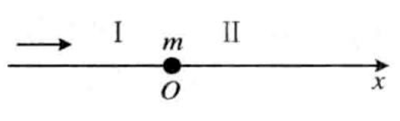
\includegraphics[width=0.3\linewidth,height=0.6\textheight,keepaspectratio]{figures/力图7-38-1.png}\\[2pt]
\textit{力图7-38-1}
\end{tabular}
\end{center}
\vfill
\newpage

\textbf{7-39} 音叉与频率为 $250.0\mathrm{Hz}$ 的标准声源同时发音时，产生 $1.5\mathrm{Hz}$ 的拍音。当音叉粘上一小块橡皮泥时，拍频增加了。如力图7-39-1，将该音叉放在盛水的细管口，连续调节水面的高度，当空气柱高度相继为 $0.34\mathrm{m}$ 和 $1.03\mathrm{m}$ 时发生共振。

试求:

1. 声波在空气中的声速.

2. 画出空气柱中的驻波图.



\begin{center}
\begin{tabular}{c}
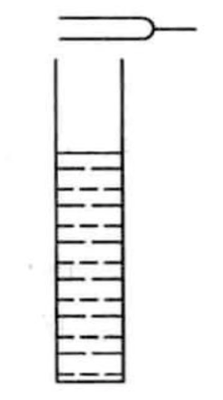
\includegraphics[width=0.3\linewidth,height=0.6\textheight,keepaspectratio]{figures/力图7-39-1.png}\\[2pt]
\textit{力图7-39-1}
\end{tabular}
\end{center}
\vfill
\newpage

\textbf{7-40} 小提琴弦长为 $L$ ，质量线密度为 $\rho$ ，张力为 $T.1$ 。用手指轻按弦的中点，试求基频和一次谐波的频率，并写出弦上各点的振动方程式。2. 在弦的一端 $\frac{L}{3}$ 长度上均匀包缠细线，使其线密度增加为 $4\rho$ ，放开手指，试求基频，并写出弦上各点的振动表达式。
\vfill
\newpage

\textbf{7-41} 一列振幅为 $A$ ，频率为 $\nu$ ，波长为 $\lambda$ 的横波沿一拉紧的水平细线传播。细线单位长度的质量为 $\rho$ 。任一点位移的表达式为
$$
y _ {1} = A \sin 2 \pi \left(\nu t - \frac {x}{\lambda}\right)
$$

式中 $t$ 为时间, $x$ 为细线上各点的水平坐标.

另一列具有相同振幅、频率、波长的波同时在细线中沿相反方向传播。两列波 $t = 0$ 时在 $x = 0$ 处的相位差为 $\varphi$ 。今在 $x = 0$ 和 $x = L$ 两处将细线固定。

1. 试导出细线中的驻波方程，并求细线中所有可能存在的波长。

2. 试求任意时刻的总动能和总势能，规定细线上各点均处于平衡位置时的总势能为零点。

3. 设 $L = 2.50 \mathrm{~m}$ , 长为 $L$ 的细线的质量为 $m = 0.0100 \mathrm{~kg}$ , 细线中的张力 $T = 10.0 \mathrm{~N}$ , 驻波的最大振幅为 $0.02 \mathrm{~m}$ . 

(a) 试求基模的频率和对应的总能量. 

(b) 用手拨动细线, 在其中激起所有可能的驻波模式, 然后在距端点 $0.50 \mathrm{~m}$ 处抓住细线. 试问哪些频率的驻波可在细线中继续存留.
\vfill
\newpage

\textbf{7-42} 飞机在上空以速度 $v = 200\mathrm{m / s}$ 作水平飞行，发出频率为 $\nu_{0} = 2000\mathrm{Hz}$ 的声波。静止在地面上的观察者测定飞机发出的声波的频率，当飞机越过观察者上空时，观察者在 $4\mathrm{s}$ 钟内测出的频率从 $\nu_{1} = 2400\mathrm{Hz}$ 降为 $\nu_{2} = 1600\mathrm{Hz}$ 。已知声波在空气中的速度为 $v = 330\mathrm{m / s}$ ，试求飞机的飞行高度 $h$ 。

\begin{center}
\begin{tabular}{c}
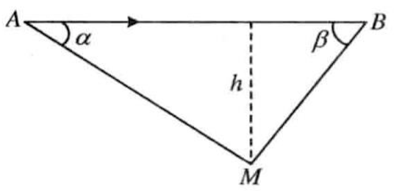
\includegraphics[width=0.3\linewidth,height=0.6\textheight,keepaspectratio]{figures/力图7-42-1.png}\\[2pt]
\textit{力图7-42-1}
\end{tabular}
\end{center}
\vfill
\newpage

\textbf{7-43} 如图，音叉 $P$ 沿着半径 $r = 8\mathrm{m}$ 的圆以角速度 $\omega = 4\mathrm{rad / s}$ 作匀速圆周运动。音叉发出频率为 $\nu_{0} = 500\mathrm{Hz}$ 的声波，声波的速度为 $v = 330\mathrm{m / s}$ 。观测者 $M$ 与圆周共面，与圆心 $O$ 的距离为 $d = 2r$ 。试问当 $\theta$ 角为多大时，观测到的频率为最高或最低，并求其数值。 $\theta$ 是 $OP$ 和 $OM$ 的夹角。



\begin{center}
\begin{tabular}{c}
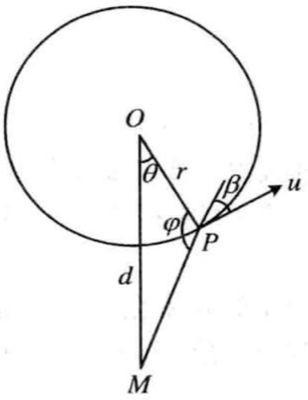
\includegraphics[width=0.3\linewidth,height=0.6\textheight,keepaspectratio]{figures/力图7-43-1.png}\\[2pt]
\textit{力图7-43-1}
\end{tabular}
\end{center}
\vfill


\end{document}
